% !TeX root = ../main.tex

\chapter{系統設計}
自主身分(AID)是\textbf{由使用者個人裝置管理的網路唯一身份},其核心理念在於讓每位使用者在具備\textbf{動態道德標準}的身分系統中\textbf{自由的管理自己},從而解決現有身分管理系統的問題。本章節將深入探討如何通過核心機制的設計將這一理念融入系統中,同時闡述系統的完整架構設計、資安與隱私議題和資料結構,為AID系統的實際應用奠定理論基礎。
\section{系統的新設計}
Yuxuan\cite{ntu-lin2014autonomous}提出的AID系統可概括為三個核心設計:自主認證、數據自主性和信用評分機制。本節將擴展前人對「自主」的概念理解,從「使用者能夠完全掌控自己的數據和隱私」深化為「讓每位使用者在具備動態道德標準的身分系統中自由管理自我」。同時也會直面身份系統與自主性之間難以迴避的矛盾:「身份本質上是為了互動而存在,但AID又希望使用者能夠完全掌控自己的數據和隱私」,提出經過縝密取捨後的新設計。
\subsection{自主認證}
自主認證是AID系統的核心,畢竟如果使用者連登入都被其他人掌握,那麼談何自主。使用者認證流程的本質可以被理解為使用者向驗證方證明「認證因素」\cite{AlQahtani2021AF}的擁有權。
\subsubsection{最簡自主認證}
本研究首先提出可以利用以下函數定義描述認證流程的本質:
\begin{itemize}
  \item Function Definitions:
        \begin{itemize}
          \item generate: $\emptyset \rightarrow (AID, token)$
          \item verify: $(AID, token) \rightarrow \{0,1\}$ \hfill // 0: fail, 1: pass
        \end{itemize}
  \item System relationship:
        \begin{itemize}
          \item $\forall(AID, token) = \text{generate}()$
          \item $\text{verify}(AID, token) = 1$
        \end{itemize}
\end{itemize}
這個函數定義了一個認證的過程,使用者可以通過generate函數獲取一個AID和token,AID被視作自主身份系統內的唯一識別號,而token伴隨AID產生,可以作為AID的認證因素。因此verify函數只要檢測到token和AID的對應關係即可通過認證。

傳統身分管理系統的認證模式雖然能滿足基本需求,但在自主認證的背景下顯得不夠完善。自主認證期望使用者能夠在個人裝置上獨立管理認證因素,無需依賴外部系統完成身份驗證。這意味著認證所需的敏感信息(即token)應當留存在使用者設備內,而非傳送至其他地方。

基於這一理念,本研究提出了一個新的模型,用以描述自主認證的最基本流程:
\begin{itemize}
  \item Function Definitions:
        \begin{itemize}
          \item generate: $\emptyset \rightarrow (AID, token)$
          \item proof: $token \rightarrow one\text{-}time\text{-}proof$
          \item verify: $(AID, one\text{-}time\text{-}proof) \rightarrow \{0,1\}$ \hfill // 0: fail, 1: pass
        \end{itemize}
  \item System relationship:
        \begin{itemize}
          \item $\forall(AID, token) = \text{generate}()$
          \item $\forall one\text{-}time\text{-}proof = \text{proof}(token)$
          \item $\text{verify}(AID, one\text{-}time\text{-}proof) = 1$
        \end{itemize}
\end{itemize}
模型中引入了proof函數,它能將token轉換為一次性的驗證證明。這一機制使得使用者可以在不直接暴露token的前提下完成身份認證。成功地在保障使用者隱私和實現有效認證之間取得了平衡。

\begin{figure}
  \centering
  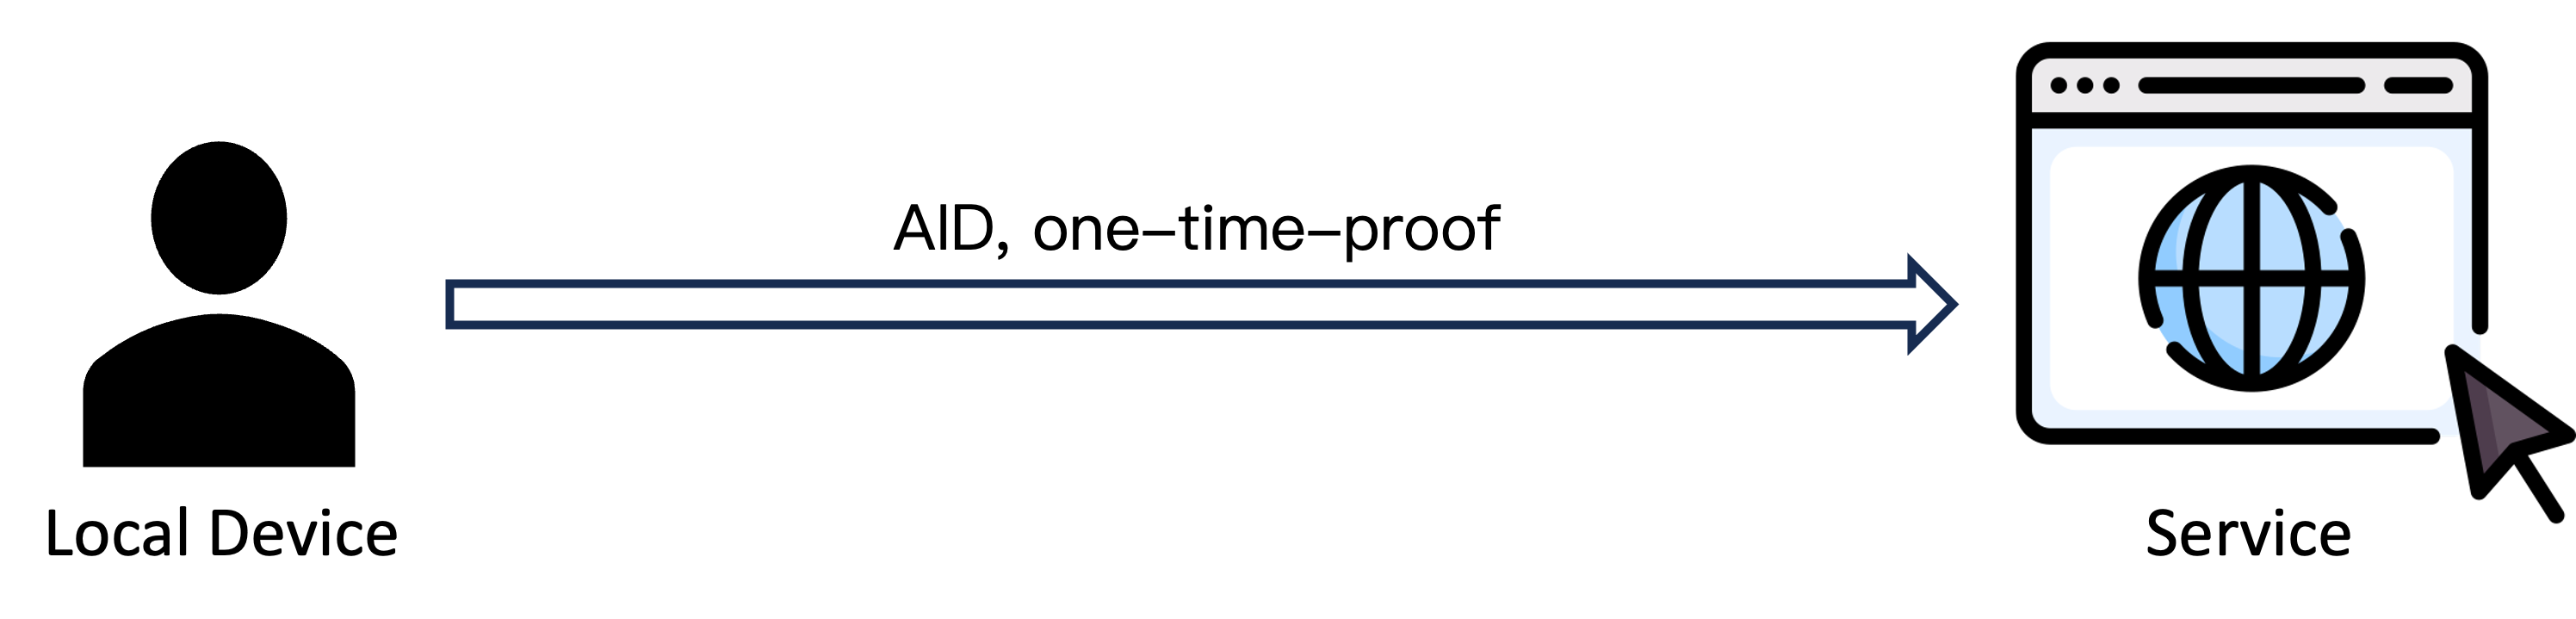
\includegraphics[width=\linewidth]{figures/min-aid.png}
  \caption{最簡自主認證}
  \label{fig:min-aid}
\end{figure}
基於前述推演,本研究提出了一個符合AID價值觀的最簡認證方案(如圖\ref{fig:min-aid}所示)。這個方案實現了在不暴露完整認證因素的情況下進行身份驗證,從而達成自主認證的核心目標。

在實際應用中,這一方案可通過多種技術來實現,如公私鑰對系統或零知識證明等。舉例來說,一種簡單的實作方式是:
\begin{itemize}
  \item 將公鑰視為AID
  \item 將私鑰視為token
  \item 使用私鑰對隨機數進行簽名,並將簽名作為one-time-proof
\end{itemize}
\subsubsection{MFA的加入}
雖然前述的最小設計為自主認證奠定了基礎,但面對當今身份管理領域的複雜挑戰,其局限性日益顯現。Bonneau等人\cite{bonneau2012mfa}的研究強調,單一認證方式(如私鑰或帳密)已無法應對現今嚴峻的安全威脅。多因素認證(Multi-Factor Authentication,MFA)因此成為必要。這一觀點得到了權威機構的廣泛認可,其中美國國家標準暨技術研究院(NIST)在其指南中明確強調了MFA的關鍵作用\cite{NIST800-63-3}。

基於這些考量,本研究提出了一個更為全面的自主認證方案模型。這個進階模型不僅保留了原有的自主性特徵,還支持多種認證因素的整合,為使用者提供了更強大的身份保護。
\begin{itemize}
  \item Function Definitions:
        \begin{itemize}
          \item generate: $\emptyset \rightarrow (AID)$
          \item bind: $(AID, token) \rightarrow AID$
          \item proof: $token \rightarrow one\text{-}time\text{-}proof$
          \item verify: $(AID, one\text{-}time\text{-}proof) \rightarrow \{0,1\}$ \hfill // 0: fail, 1: pass
        \end{itemize}
  \item System relationship:
        \begin{itemize}
          \item $\forall one\text{-}time\text{-}proof = \text{proof}(token)$
          \item $\text{verify}(\text{bind}(AID, token), one\text{-}time\text{-}proof) = 1$
        \end{itemize}
\end{itemize}
本研究提出的改進模型在原有基礎上做出了兩項關鍵調整:首先,將AID的生成過程獨立化;其次,引入了bind函數,用於將不同的認證因素(token)綁定到AID上,從而實現多因素認證(MFA)。

然而,這種看似完善的設計卻帶來了新的挑戰,主要體現在系統複雜度的增加。在現有密碼學技術框架下,要在數學上嚴格證明某個認證因素與獨立生成的AID之間的關聯性仍然困難重重。因此,實現這一模型往往需要依賴更為複雜的系統設計和實作。

值得一提的是,Wang等人\cite{Wang2013ThresholdSignatureSchemes}提出的門限簽名方案為解決這一問題提供了一個潛在途徑。該方案允許在生成單一公鑰的同時產生多個私鑰,理論上可以在不需額外bind機制的情況下實現上述模型。然而,這種方案在實際應用中面臨諸多限制,難以被視為MFA的完整解決方案。
\subsubsection{AID Server的加入}
\begin{figure}
  \centering
  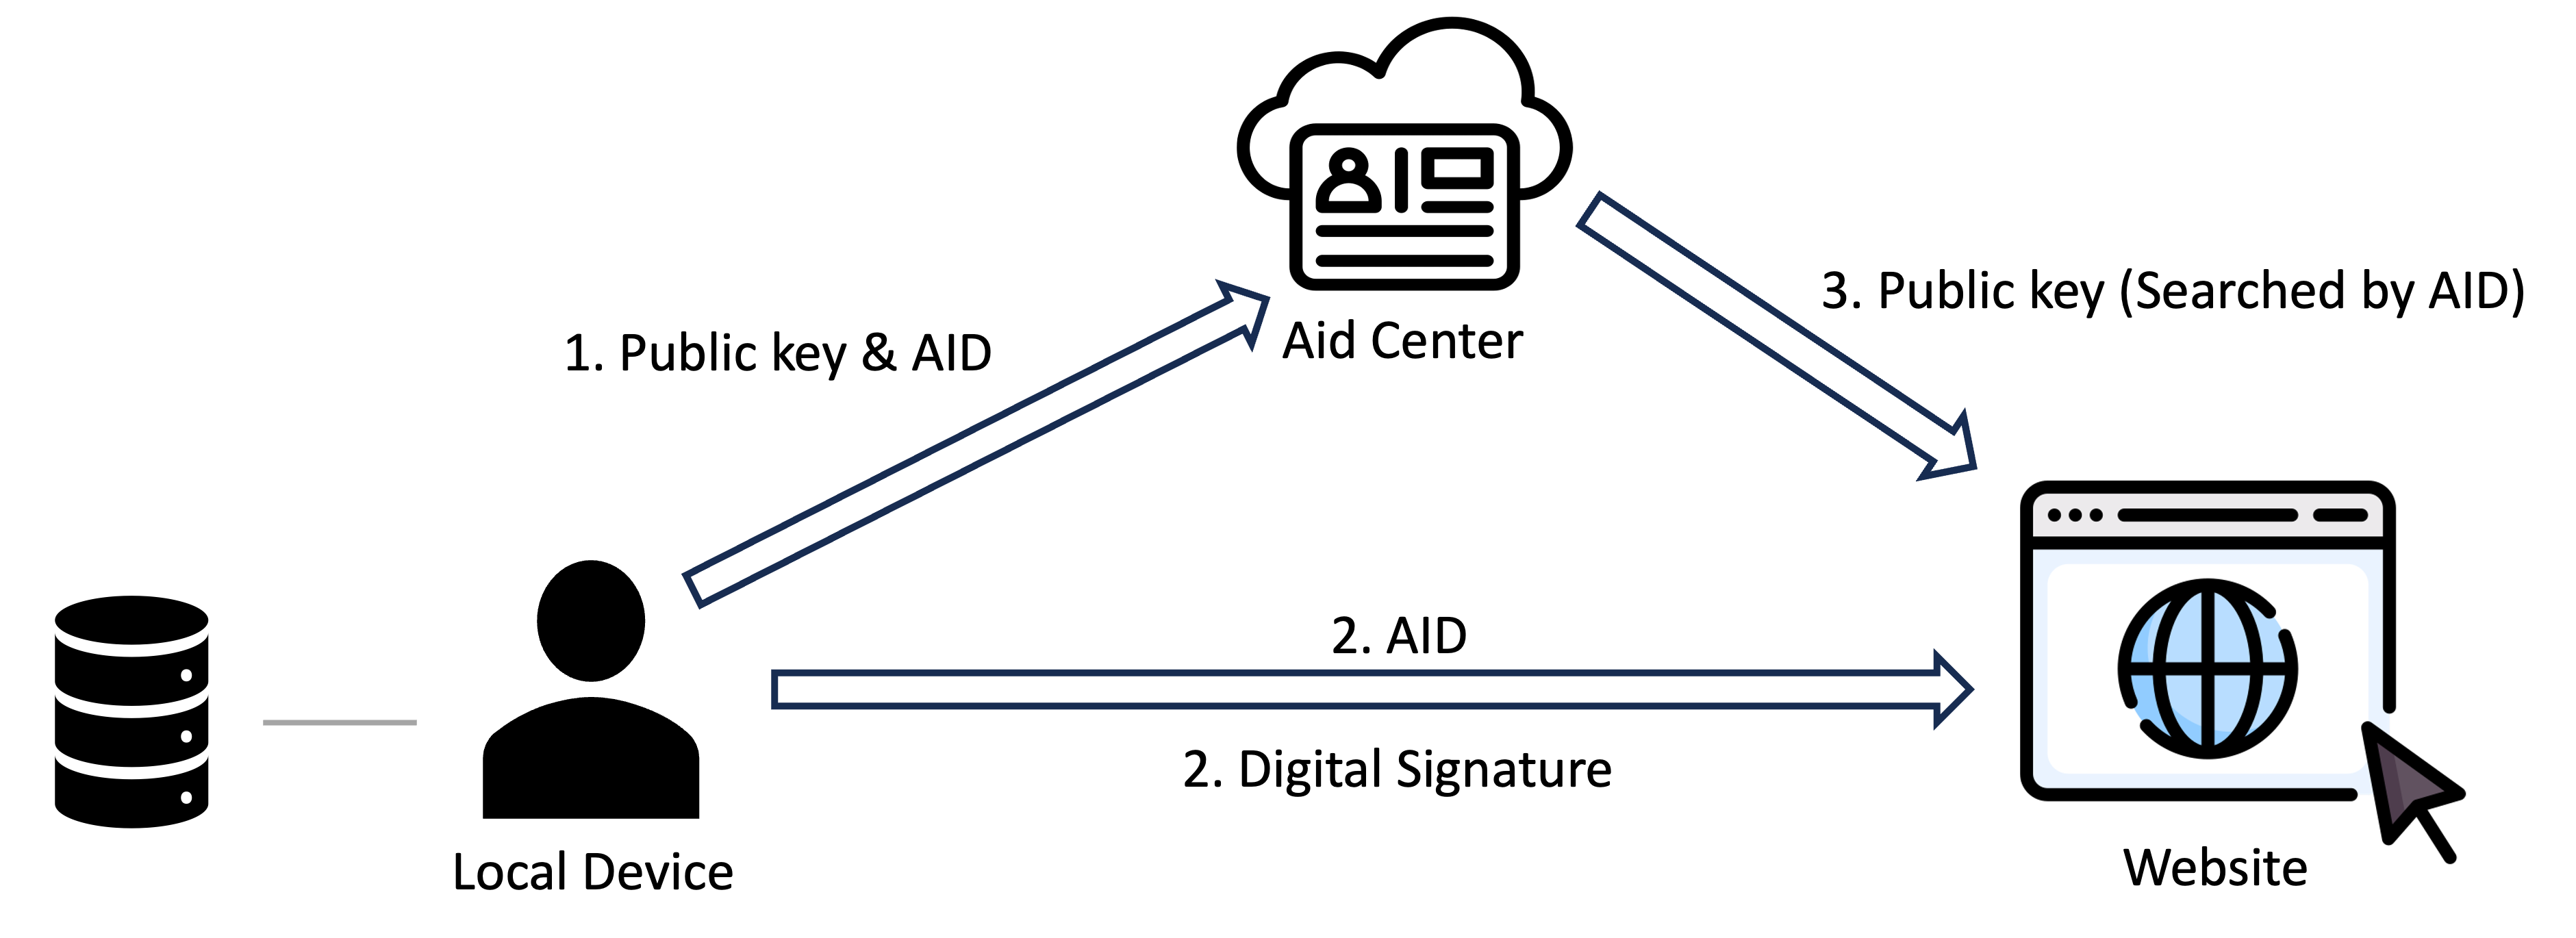
\includegraphics[width=\linewidth]{figures/old-aid-login.png}
  \caption{過去的自主認證}
  \label{fig:old-aid-login}
\end{figure}
Yuxuan設計的AID系統\cite{ntu-lin2014autonomous}可被視為前述模型的一個實際實現(如圖\ref{fig:old-aid-login})。該系統的核心機制如下:
\begin{enumerate}
  \item \textbf{產生ID:}使用者在個人裝置上生成UUID\cite{uuid}作為唯一識別號。
  \item \textbf{產生認證因素:}由於UUID本身不具備可認證特性,使用者還需在裝置上生成一對公私鑰。
  \item \textbf{連結認證因素:}將公鑰與UUID一同上傳至中心化AID Server,建立連結。
  \item \textbf{身份認證:}認證時,使用者通過私鑰對隨機數據進行簽名,驗證者則可從AID Server獲取對應UUID的公鑰來驗證簽名。
\end{enumerate}
這種設計不僅實現了基本的身份認證功能,還通過中心化的AID Server巧妙解決了兩個關鍵安全問題:
\begin{itemize}
  \item \textbf{ID重複問題:} 儘管UUID重複的機率極低,但在實際場景中,惡意使用者可能刻意生成相同的UUID,導致身份混淆。AID Server通過確保每個傳入的UUID的唯一性,有效防止了這一問題,拒絕任何重複UUID的綁定請求。
  \item \textbf{身份強佔問題:} 作為ID重複問題的延伸,身份強佔指惡意使用者可能在UUID真實擁有者使用特定服務前,搶先綁定該UUID,致使真實擁有者無法使用服務。AID Server通過在使用者進入服務時驗證UUID與公鑰的對應關係,有效規避了這一風險。
\end{itemize}

深入探討上述流程,本研究發現了一些問題,首先,中心化的AID Server雖然解決了ID重複問題與身份強佔問題,但是卻導致了新的問題如\textbf{單點故障}、\textbf{可擴展性}等。其次,中心化的AID Server也無法滿足AID系統的最初目標:\textbf{自主認證}。使用者無法完全自主管理自己的身份,而是需要依賴中心化的AID Server提供的連結能力才能完成認證。為了解決這些問題,本研究提出以下原則希望能夠重新設計AID系統:
\begin{itemize}
  \item \textbf{去中心化}:把區塊鏈技術應用到AID系統的實作中,從而消除中心化的AID Server,實現系統的高可用性和可信任。
  \item \textbf{去依賴性}:使用者認證時不應該要求服務到AID Server搜索綁定UUID的公鑰,而應該是讓使用者自主宣告綁定的公鑰等關聯認證因素,AID Server只負責記錄這個宣告,作為額外的保證。
\end{itemize}
\subsubsection{自主憑證的使用}
最後,單純的加入區塊鏈技術取代AID Server並不是沒有缺點,除了區塊鏈技術的性能限制外,還有一個更為重要的問題:\textbf{隱私}。區塊鏈技術的特性決定了所有的交易都是公開的,這將導致使用者的綁定關係被公開,進而影響使用者的隱私。過去的設計中僅使用公鑰作為綁定因素尚無隱私問題,但MFA機制中常用的手機驗證碼、信箱驗證碼等都是私密資訊,這樣的設計將導致使用者的隱私受到威脅。

\begin{figure}
  \centering
  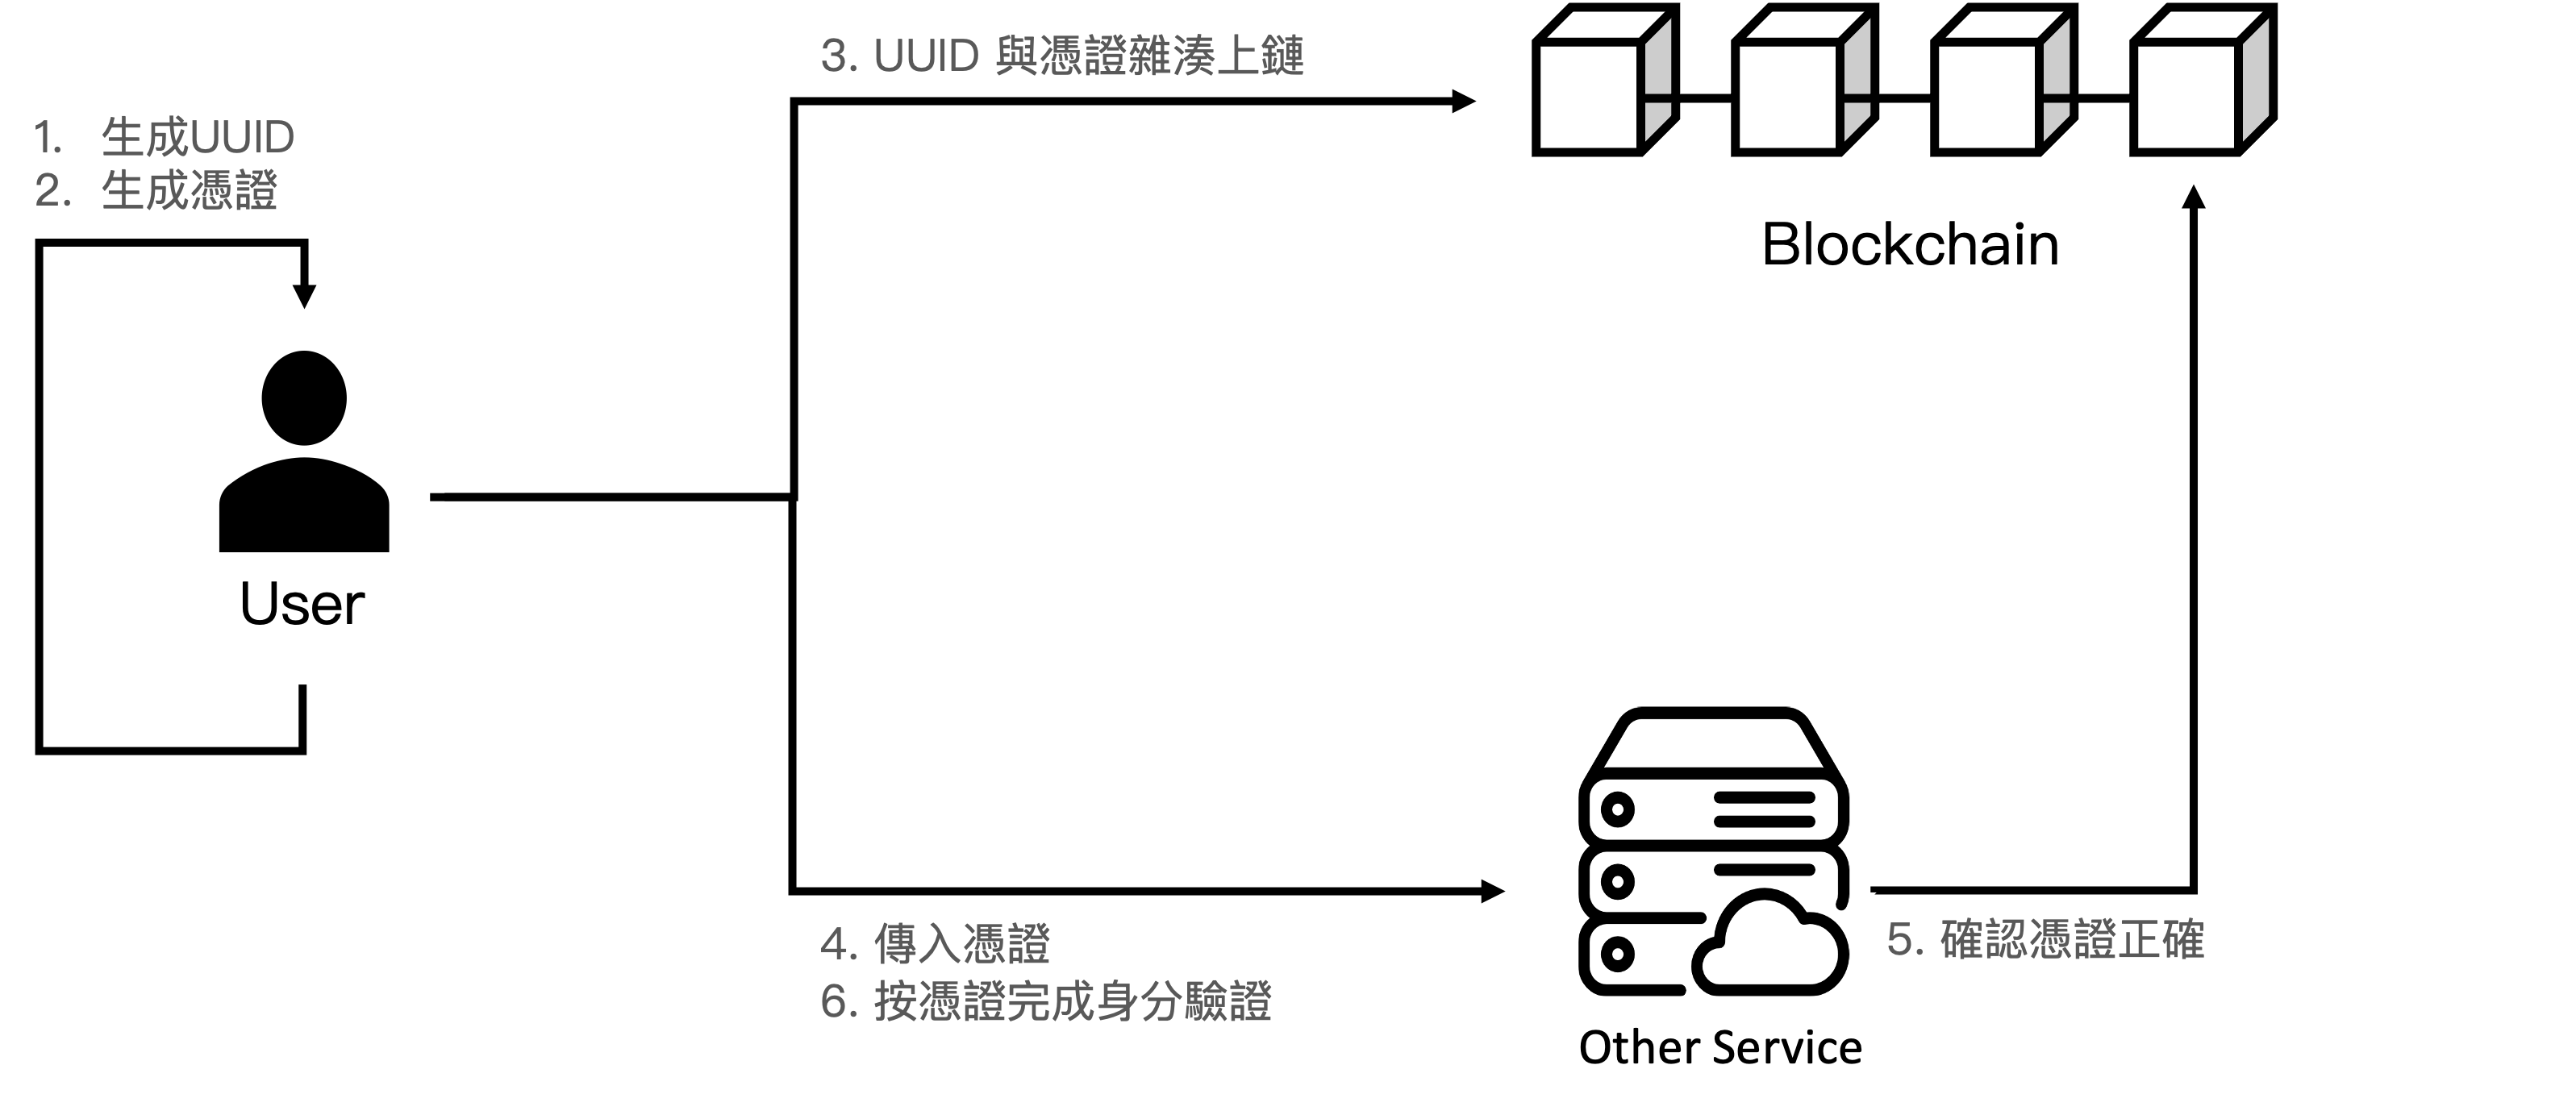
\includegraphics[width=\linewidth]{figures/new-aid-login.png}
  \caption{自主認證(加入憑證機制)}
  \label{fig:new-aid-login}
\end{figure}
為解決前述挑戰,本研究對Tze-Nan\cite{NTU202102846}提出的「自主憑證」概念進行了簡化和優化。如圖\ref{fig:new-aid-login}所示,新的自主認證解決方案建立在一個新機制上。在這個機制中,使用者首先將個人資訊和多因素認證(MFA)所需的驗證資訊整合到類似x509的憑證結構中。隨後,系統計算該憑證結構的雜湊值,並將其上傳至區塊鏈。當使用者需要登入時,他們只需向登入對象提供完整憑證。登入對象則通過區塊鏈驗證憑證的完整性,一旦驗證通過,使用者就能用憑證中提供的MFA方案和資訊完成登入程序。另外,如果使用者在憑證內的個人資訊需要有第三方背書,可以透過追加簽章服務後在憑證內部加入第三方簽章來完成。

這種設計極大地增強了系統的安全性和隱私保護能力。首先,由於使用者自行保管包含個人資料和驗證資訊的完整憑證,個人隱私得到了有效保護。其次,區塊鏈僅存儲憑證的雜湊值和使用者的UUID,大幅減少了敏感資訊外洩的風險,實現了資料最小化原則。再者,通過區塊鏈驗證憑證完整性,結合MFA機制,確保了整個認證過程的安全可靠。最重要的是,這個方案賦予了使用者更大的自主權,使他們能夠自主決定何時、向誰提供憑證,從而增強了對個人身份資訊的掌控。
\subsubsection{自主認證的流程}
這個優化後的「自主認證」方案不僅有效平衡了隱私保護和認證安全性,還為使用者提供了更大的身份資訊自主權,充分體現了AID系統的核心理念。以下深入描述這個方案的細節流程:
\begin{enumerate}
  \item 使用者在個人設備上:
        \begin{enumerate}
          \item 產生 UUID
          \item 選擇認證因素(如手機、信箱、金鑰等)
          \item 將對應資訊(如手機號碼、信箱地址、公鑰等)加入憑證
        \end{enumerate}

  \item 憑證處理:
        \begin{enumerate}
          \item 填入欲揭露的個人資訊(類似過去 AID 中的 actor profile)
          \item 計算憑證的雜湊值
          \item 將雜湊值上傳至區塊鏈
        \end{enumerate}

  \item 登入流程:
        \begin{enumerate}
          \item 使用者將憑證傳送給登入對象
          \item 登入對象在區塊鏈中透過檢查雜湊值驗證憑證的完整性
          \item 登入對象要求使用者使用憑證內的驗證方案完成認證
          \item 使用者依要求完成認證(例如:使用私鑰對隨機數進行簽名來證明擁有公鑰)
        \end{enumerate}
\end{enumerate}
\subsection{數據自主}
\begin{figure}
  \centering
  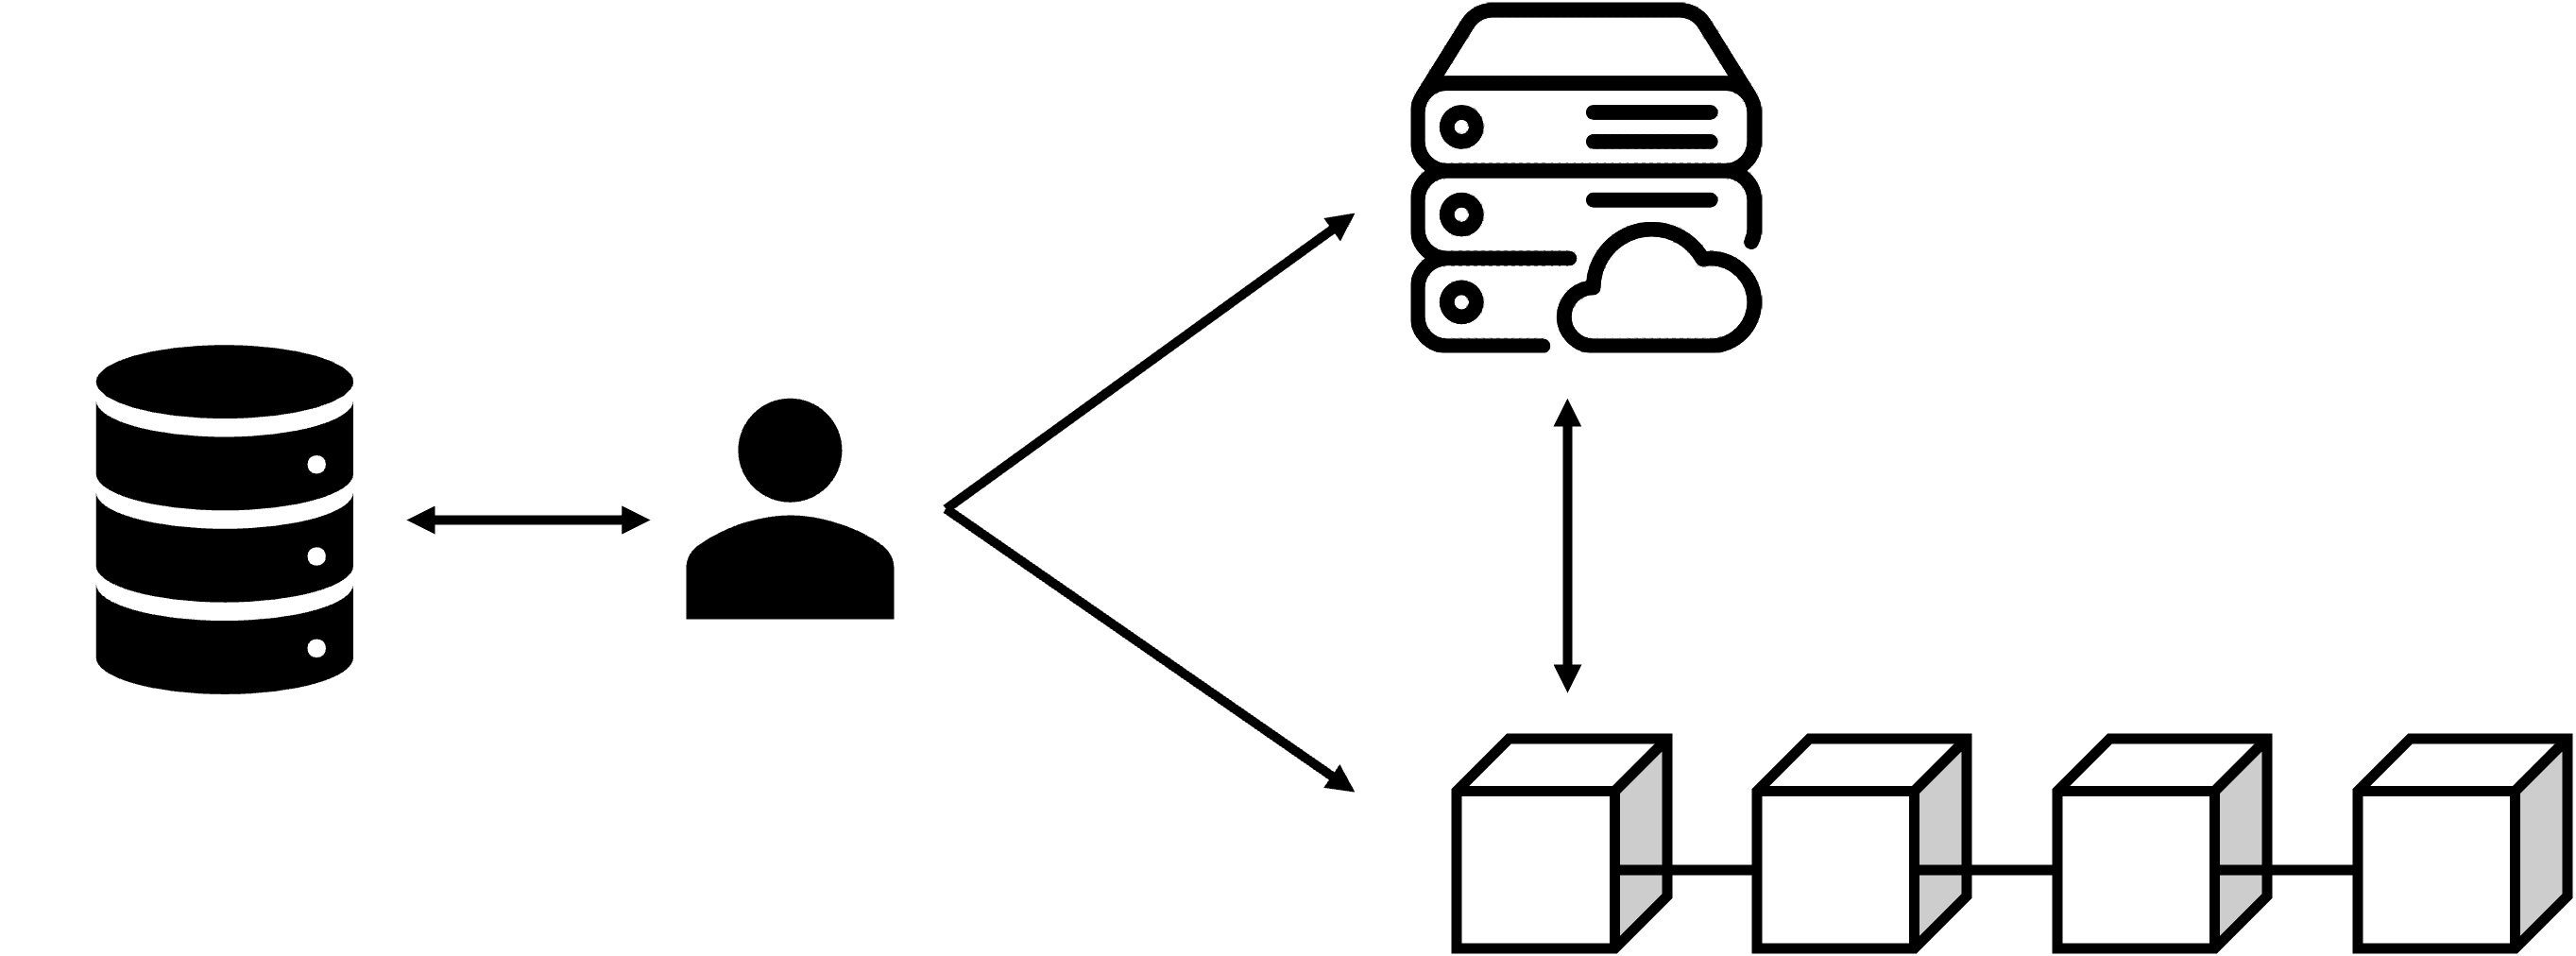
\includegraphics[width=\linewidth,keepaspectratio]{figures/aid.png}
  \caption{自主身分}
  \label{fig:aid}
\end{figure}
實現數據的自由管理是一項具有挑戰性的任務。在傳統身分管理系統中,使用者數據通常由身分供應商(Identity Provider)或服務提供商(Service Provider)集中控制,這嚴重限制了使用者在個人數據上的自由。為了克服這一限制,AID系統採用了獨特的「數據層反轉」策略如圖\ref{fig:aid}:將使用者數據完全遷移至使用者端設備,從而實現使用者對個人數據的直接控制。

\begin{figure}
  \centering
  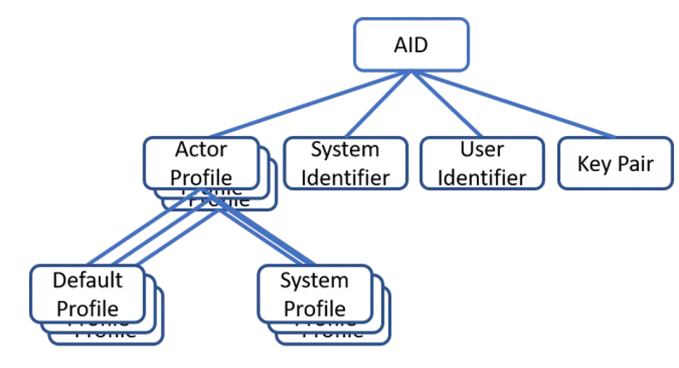
\includegraphics[width=\linewidth]{figures/old-aid-struct.png}
  \caption{過去的AID資料結構}
  \label{fig:old-aid-struct}
\end{figure}
更深入的描述,在過去的AID系統中,在個人裝置保留角色資料(actor profile)的資料結構(如圖\ref{fig:old-aid-struct})。其中,每個角色資料包含了一組預設資料與多組服務資料。預設資料是使用者自行提供的基本資料,如姓名、性別、年齡等。服務資料則是使用者在使用各服務時產生的資料,如交易記錄、行為日誌等。設計上,盡可能在個人裝置上使用服務,當不得不上傳資料時,使用者可以選擇上傳哪個角色的哪組資料,從而實現數據的自主權。

然而,本研究認為這樣的設計僅實現了GDPR\cite{GDPR2016}中強調的「數據最小揭露」,並沒有完整面對數據自主背後的艱困挑戰。就像蘋果公司AI服務\cite{apple_foundation_models}的隱私困境,AI模型需要讀取使用者的隱私才能更好的協助使用者。確實存在著理想的做法,就是只使用個人設備內的小型AI模型產生推論,而不是將所有數據上傳到雲端進行運算。但是,這樣的做法在實際應用中卻面臨著巨大的挑戰,因為小型AI模型的能力有限,無法滿足複雜的應用需求。因此,蘋果公司會在個人設備的小型AI模型無法妥善處理的情況下,使用特殊的私有雲計算方案\cite{apple_private_cloud_compute}來保護使用者的隱私。

\begin{table}
  \centering
  \begin{tabular}{>{\raggedright\arraybackslash}p{2.5cm}>{\raggedright\arraybackslash}p{2.5cm}>{\raggedright\arraybackslash}p{4cm}>{\raggedright\arraybackslash}p{4cm}}
    \toprule
    \textbf{挑戰}                         & \textbf{說明}       & \textbf{關鍵概念} & \textbf{技術解決方案} \\
    \midrule
    數據被遺忘權                              & 使用者有權要求完全刪除其個人數據  &
    \begin{itemize}[nosep,leftmargin=*]
      \item 分散存儲帶來的挑戰
    \end{itemize} &
    \begin{itemize}[nosep,leftmargin=*]
      \item 無狀態服務
      \item 數據不可定向性
    \end{itemize}                                                        \\
    \addlinespace
    數據明確授權                              & 收集數據前需獲得明確同意並說明用途 &
    \begin{itemize}[nosep,leftmargin=*]
      \item 目的明確原則
      \item 使用者體驗設計
      \item 使用者認知負擔
    \end{itemize} &
    \begin{itemize}[nosep,leftmargin=*]
      \item 數據憑證機制
      \item 數據流動的透明化
    \end{itemize}                                                        \\
    \addlinespace
    數據可驗證性                              & 確保數據的正確性和一致性      &
    \begin{itemize}[nosep,leftmargin=*]
      \item 跨服務數據傳遞流程
      \item 去中心化帶來的挑戰
    \end{itemize} &
    \begin{itemize}[nosep,leftmargin=*]
      \item 數據憑證機制
      \item 區塊鏈智能合約
    \end{itemize}                                                        \\
    \addlinespace
    無特權的執行                              & 減少對特權管理者的依賴       &
    \begin{itemize}[nosep,leftmargin=*]
      \item 使用者自主管理
      \item 便利性與責任平衡
    \end{itemize} &
    \begin{itemize}[nosep,leftmargin=*]
      \item 極限多因素驗證
      \item 暫時提權方案
    \end{itemize}                                                        \\
    \bottomrule
  \end{tabular}
  \caption{數據自主的四個難題}
  \label{tab:aid-data-difficult}
\end{table}
基於這樣的背景,本研究提出數據自主權應考慮到\textbf{不得不上傳的數據}與\textbf{直接由服務產生的個人數據},並直接面對表\ref{tab:aid-data-difficult}幾個關鍵挑戰。
\subsubsection{數據被遺忘權}
數據被遺忘權(Right to be Forgotten)是現代數據保護法規中的一項關鍵原則,它賦予使用者要求服務供應商完全刪除其個人數據的權利。然而,在技術實現層面,這個看似簡單的要求卻面臨著巨大的挑戰。實現數據被遺忘權的主要技術難點在於使用者資料通常以各種形式分散存儲在系統的不同部分,包括主資料庫、日誌系統、備份存儲等\cite{smirnova2024understanding}。此外,某些數據可能與其他使用者的數據或系統日誌緊密關聯,難以單獨刪除。

為了應對這些挑戰,本研究提出了結合自主身份(AID)系統和無狀態服務(Stateless Service)概念的解決方案。AID系統的核心理念是將主要數據存儲在使用者個人裝置中,而非集中在服務供應商的伺服器上。這種去中心化的方法大大簡化了數據刪除的過程。與此同時,借鑒了\cite{krstic2023cloud_encryption}的研究,我們提出服務供應商應採用無狀態設計原則。在這種設計下,每次交互結束後,服務供應商會刪除與使用者相關的所有臨時數據。對於必須保留的數據(如交易記錄),則由使用者下載並自行管理,在下次使用服務時重新上傳必要的數據。

這種結合AID系統和無狀態服務的方法具有多重優勢。首先,它極大地簡化了刪除流程,因為大部分數據由使用者自行管理,服務供應商只需處理少量臨時數據。其次,這種方法顯著增強了隱私保護,降低了數據被不當收集或利用的風險。此外,它提高了整個數據處理過程的透明度,使用者能夠清楚知道哪些數據被服務存儲,哪些由自己管理。最後,這種方法更容易滿足如 GDPR 等嚴格的數據保護法規要求。

儘管無狀態服務為實現數據被遺忘權提供了有效途徑,但這種方法也引發了一系列新的挑戰,尤其是在數據信任和適用性方面。首要問題是數據的可信度。當服務要求使用者保存具有實質價值的狀態數據時,如可兌換現金的積分或重要的交易記錄,這些存儲在使用者端的數據可能面臨被惡意修改的風險。這不僅威脅到服務的正常運作,還可能給服務供應商帶來巨大的經濟損失。

為了解決這個信任問題,本研究提出了一種基於密碼學的驗證機制。這種機制的核心是利用數字簽名技術確保數據的完整性和真實性。具體而言,服務供應商會對關鍵數據的雜湊值進行加密簽名,然後將原始數據和簽名一併返回給使用者。在使用者再次使用服務時,需同時上傳數據和對應的簽名。服務供應商通過以下步驟驗證數據的完整性:
\begin{enumerate}
  \item 接收使用者上傳的數據和簽名。
  \item 使用存儲的私鑰解密簽名,獲得原始雜湊值。
  \item 對接收到的數據重新計算雜湊值。
  \item 比較解密後的雜湊值和新計算的雜湊值。
\end{enumerate}
如果兩個雜湊值相符,則可以確認數據在使用者端存儲期間未被篡改。這種方法既保證了數據的完整性,又維持了無狀態服務的核心優勢。

然而,我們必須認識到,無狀態服務並非適用於所有場景。某些應用類型,如社交網絡平台或在線論壇,其核心功能就是依賴於在平台上持續存儲和展示使用者生成的內容。對於這類應用,完全採用無狀態服務模式是不切實際的。

在這種情況下,本研究提出了一種基於「不可定向性」原則的替代方案。這一方案即使在必須保留使用者數據的情況下,也能在一定程度上保護使用者隱私。其概念是將使用者上傳的數據進行匿名化處理,使其無法直接與特定使用者關聯。具體而言,可以將使用者數據中的個人識別信息(如姓名、地址、實名AID等)替換為標識符,使用者可以單向的證明自己擁有數據,但服務沒有辦法直接證明數據與特定使用者的關聯。這種方法在一定程度上保護了使用者隱私,同時也滿足了服務的核心功能需求。

總的來說,無狀態服務雖然為數據被遺忘權提供了有力支持,但並非放之四海而皆準的解決方案。在實際應用中,需要根據具體情況選擇適當的技術方案,並在數據保護、使用者體驗和服務功能之間尋求最佳平衡點。
\subsubsection{數據明確授權}
近年來,隨著數據保護法規的不斷演進,特別是歐盟通用數據保護條例(GDPR)的實施,數據授權問題已成為企業,尤其是大型跨國企業面臨的重大挑戰之一。Saemann\cite{saemann2022investigating}的研究深入探討了GDPR實施後企業在數據管理實踐中遇到的困難,特別強調了目的明確(Purpose Specification Principle)的複雜性。企業必須在收集個人數據之前獲得數據主體的明確同意,並清晰闡明數據的使用目的和範圍。這一看似直接的要求,實則蘊含了多層次的法律和技術挑戰。

以Google和Amazon為例,這兩家公司儘管在數據收集過程中提供了全面的隱私設定選項,但仍被歐盟監管機構認定為未能充分獲得使用者的明確同意。2019年,法國國家資訊自由委員會(CNIL)對Google處以5000萬歐元的罰款,指出其隱私政策缺乏透明度和具體性\cite{CNIL_SAN-2019-001}。同樣,2021年盧森堡國家數據保護委員會(CNPD)因Amazon的廣告個性化做法違反GDPR,對其處以7.46億歐元的罰款\cite{SimmonsSimmons_AmazonGDPR}。

這些案例揭示了即便是資源豐富的科技巨頭,在實現GDPR合規性時也面臨著重大挑戰。相關判決強調,僅僅提供隱私設定選項是不夠的,關鍵在於這些選項的設計和呈現方式。具體而言,這些公司的做法之所以被認定為不符合GDPR標準,主要基於兩個方面的考量:
\begin{enumerate}
  \item \textbf{使用者體驗設計不當:} 隱私設定介面往往缺乏直觀性和易用性。複雜的選項結構和專業術語的使用增加了使用者理解和操作的難度。介面設計對使用者的隱私決策有顯著影響,不恰當的設計可能導致使用者做出與其真實意願不符的選擇。
  \item \textbf{使用者認知負擔過重:} 大多數使用者面對繁複的隱私設置時,要麼難以充分理解每個選項的含義及其潛在影響,要麼不願投入大量時間來仔細配置這些選項。即使是受過教育的使用者也可能因為認知偏差和決策疲勞而做出次優的隱私決定。
\end{enumerate}
這些問題凸顯了在設計符合GDPR要求的數據收集機制時,不僅需要考慮法律合規性,還需要從使用者角度出發,提供直觀、易用的隱私設定選項。

\begin{figure}
  \centering
  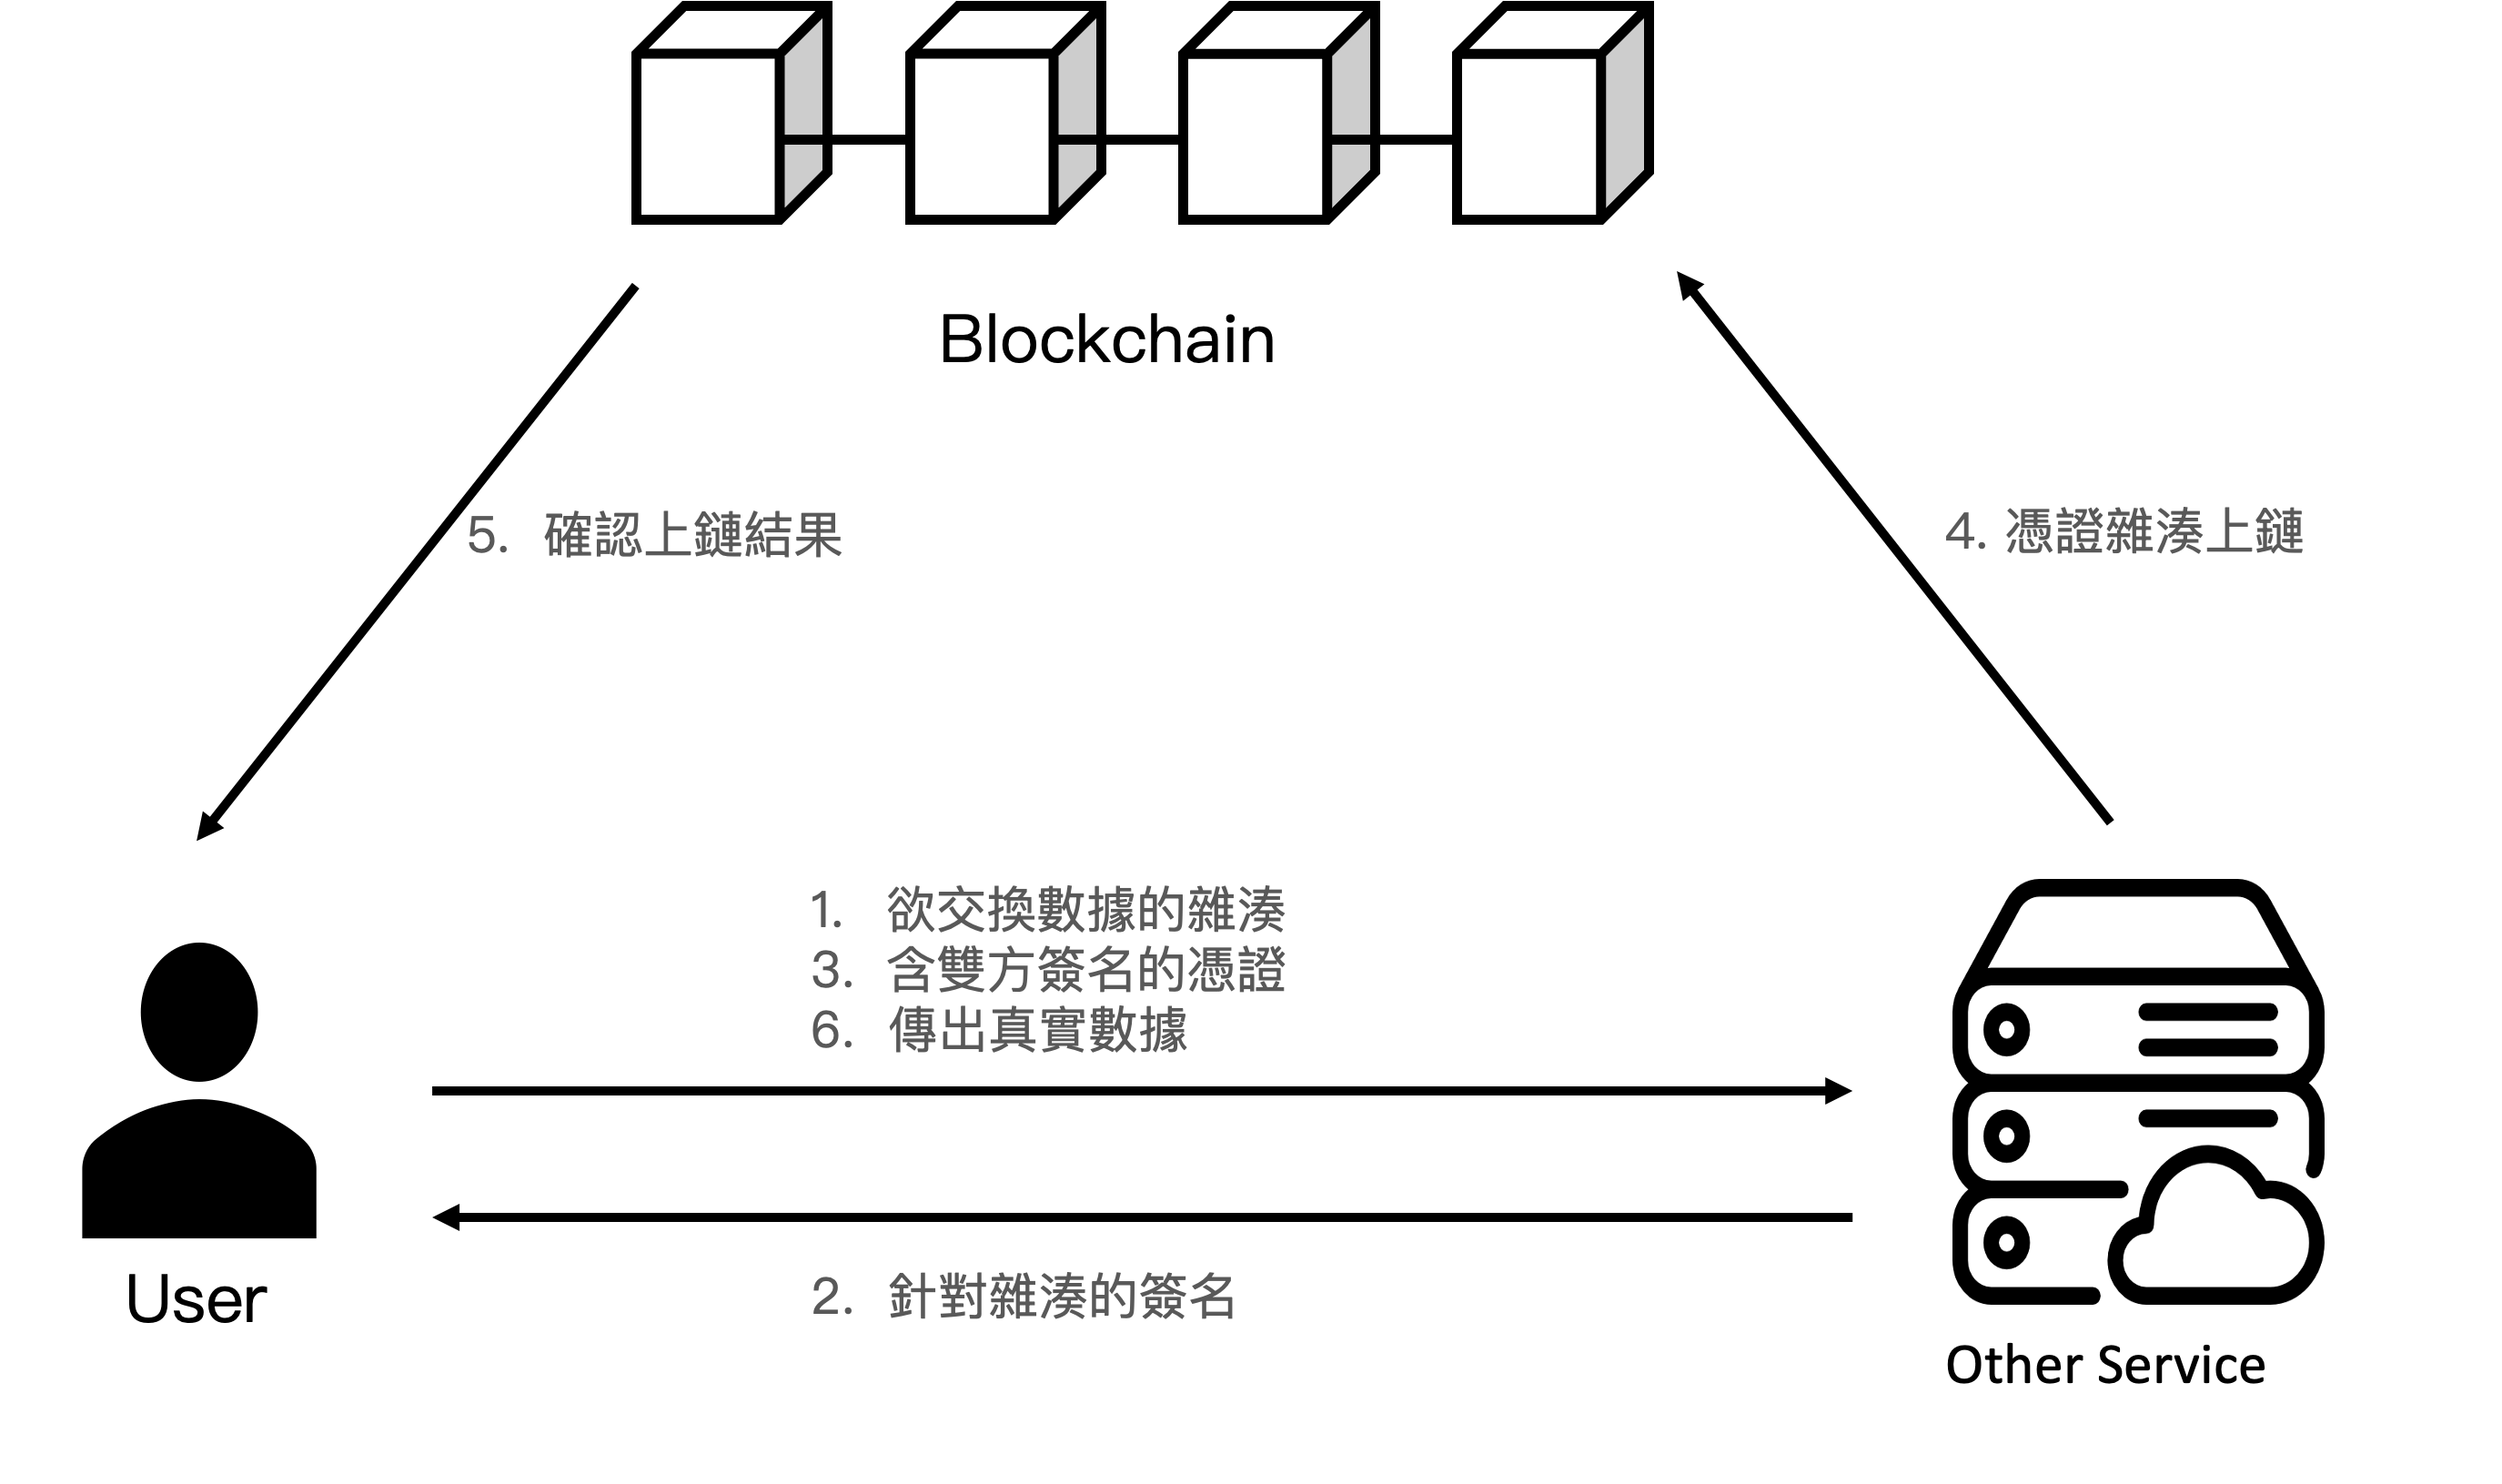
\includegraphics[width=\linewidth]{figures/min-data-perm.png}
  \caption{數據憑證(資料傳出)}
  \label{fig:min-data-perm}
\end{figure}
因此,本研究提出「數據憑證」(Data Certificate)概念(如圖\ref{fig:min-data-perm})。這一機制借鑒了自主憑證\cite{NTU202102846}的設計,為每份數據賦予一個包含多重驗證要素的電子憑證。具體而言,數據憑證包含以下關鍵元素:數據所有者的數字簽名、數據使用者的數字簽名、數據內容的加密哈希值、明確定義的使用範圍及目的。為確保憑證的不可篡改性和公開可驗證性,本研究進一步建議將憑證的雜湊值記錄於區塊鏈網絡中。

在此機制下,數據傳輸遵循嚴格的授權流程:僅當數據所有者和使用者雙方完成憑證簽署,且憑證雜湊值成功記錄於區塊鏈後,實際的數據內容才會被傳輸。這種設計明確定義了數據的內容與授權範圍,為數據使用提供了雙向保障。一方面,當發生數據濫用時,數據所有者可通過公開憑證證實濫用行為;另一方面,服務提供者也可藉由憑證證明其數據使用的合法性。結合優化的使用者互動流程,此機制有望實現更為明確和透明的數據授權過程。

此外,通過在區塊鏈上額外記錄數據特徵,本機制為個人數據流動提供了追蹤能力,從而增強了數據管理的「透明度」,這是保障隱私的關鍵環節之一。然而,值得注意的是,儘管此方法能夠明確記錄數據流動,但其有效性在很大程度上仍依賴於系統參與者的誠信和遵守規則的意願,可能在實際應用中面臨執行挑戰。鑒於此,本研究建議將數據憑證機制視為一個基礎框架,需要與其他輔助機制結合使用以增強其實際效力。例如,引入基於信用評分系統可以提升使用者對服務提供者的信任度,彌補單純依賴區塊鏈記錄的潛在不足。
\subsubsection{數據可驗證性}
在自主身份(Autonomous Identity,AID)系統中,使用者自行存儲和管理數據。這種去中心化方法雖然增強了使用者對個人數據的控制,卻也為跨服務的數據操作帶來了新的挑戰,特別是在數據的正確性(correctness)和一致性(consistency)方面。雖然數據正確性問題可以通過數位簽名技術解決,但這種方法無法解決數據一致性問題,即無法確保當前使用的數據版本是最新的,而非過時或已失效的版本。

為此,本研究提出「數據憑證」機制的不同用法,借鑒了區塊鏈在分布式系統中維護一致性的優勢。具體實施過程如下:當需要進行跨服務數據傳遞時,原始服務首先生成一個數據憑證,其中包含數據雜湊、時間戳和使用範圍等信息,並用私鑰進行簽名。隨後,原始服務將該數據憑證的雜湊值存入區塊鏈的智能合約中。這個智能合約支持即時狀態更新,確保數據的最新狀態可被追蹤。在跨服務傳遞數據時,使用者同時提供數據本身和對應的數據憑證。接收服務通過驗證憑證簽名來確認數據的正確性,並通過查詢區塊鏈上的智能合約來驗證數據的一致性。當數據發生變化時,相關服務可以即時更新智能合約的狀態,從而持續確保數據的一致性。

這種設計不僅確保了數據的「可驗證性」(Verifiability),還為AID系統中的數據提供了「可移動性」(Portability)。可驗證性使接收服務能夠驗證數據的來源、完整性和時效性,確保數據的正確性和一致性;而可移動性則允許數據在不同服務間自由傳遞,無需依賴中央認證系統,同時保持可驗證性。這種方法具有高度安全性、實時性、可審計性和隱私保護等優勢,特別適用於對數據完整性和即時性要求較高的應用場景,如金融交易系統、醫療信息交換平台和供應鏈管理系統等。

\begin{figure}
  \centering
  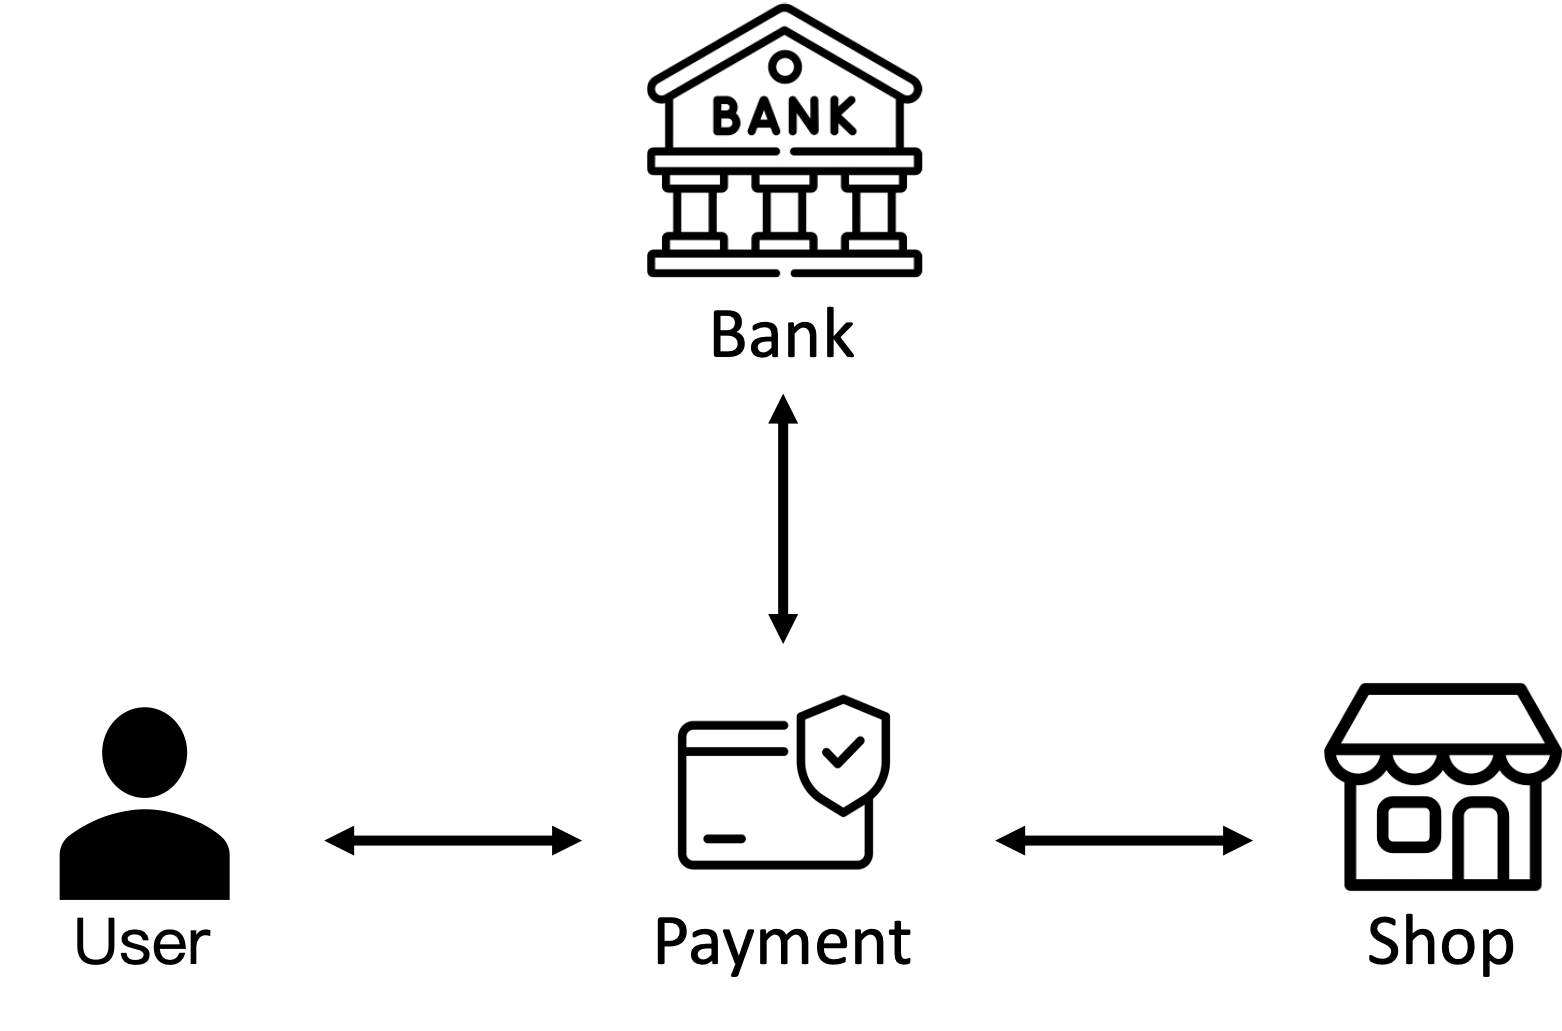
\includegraphics[width=\linewidth,keepaspectratio]{figures/flow-3-part-0.png}
  \caption{當前網路後端設計}
  \label{fig:flow-3-part-0}
\end{figure}
\begin{figure}
  \centering
  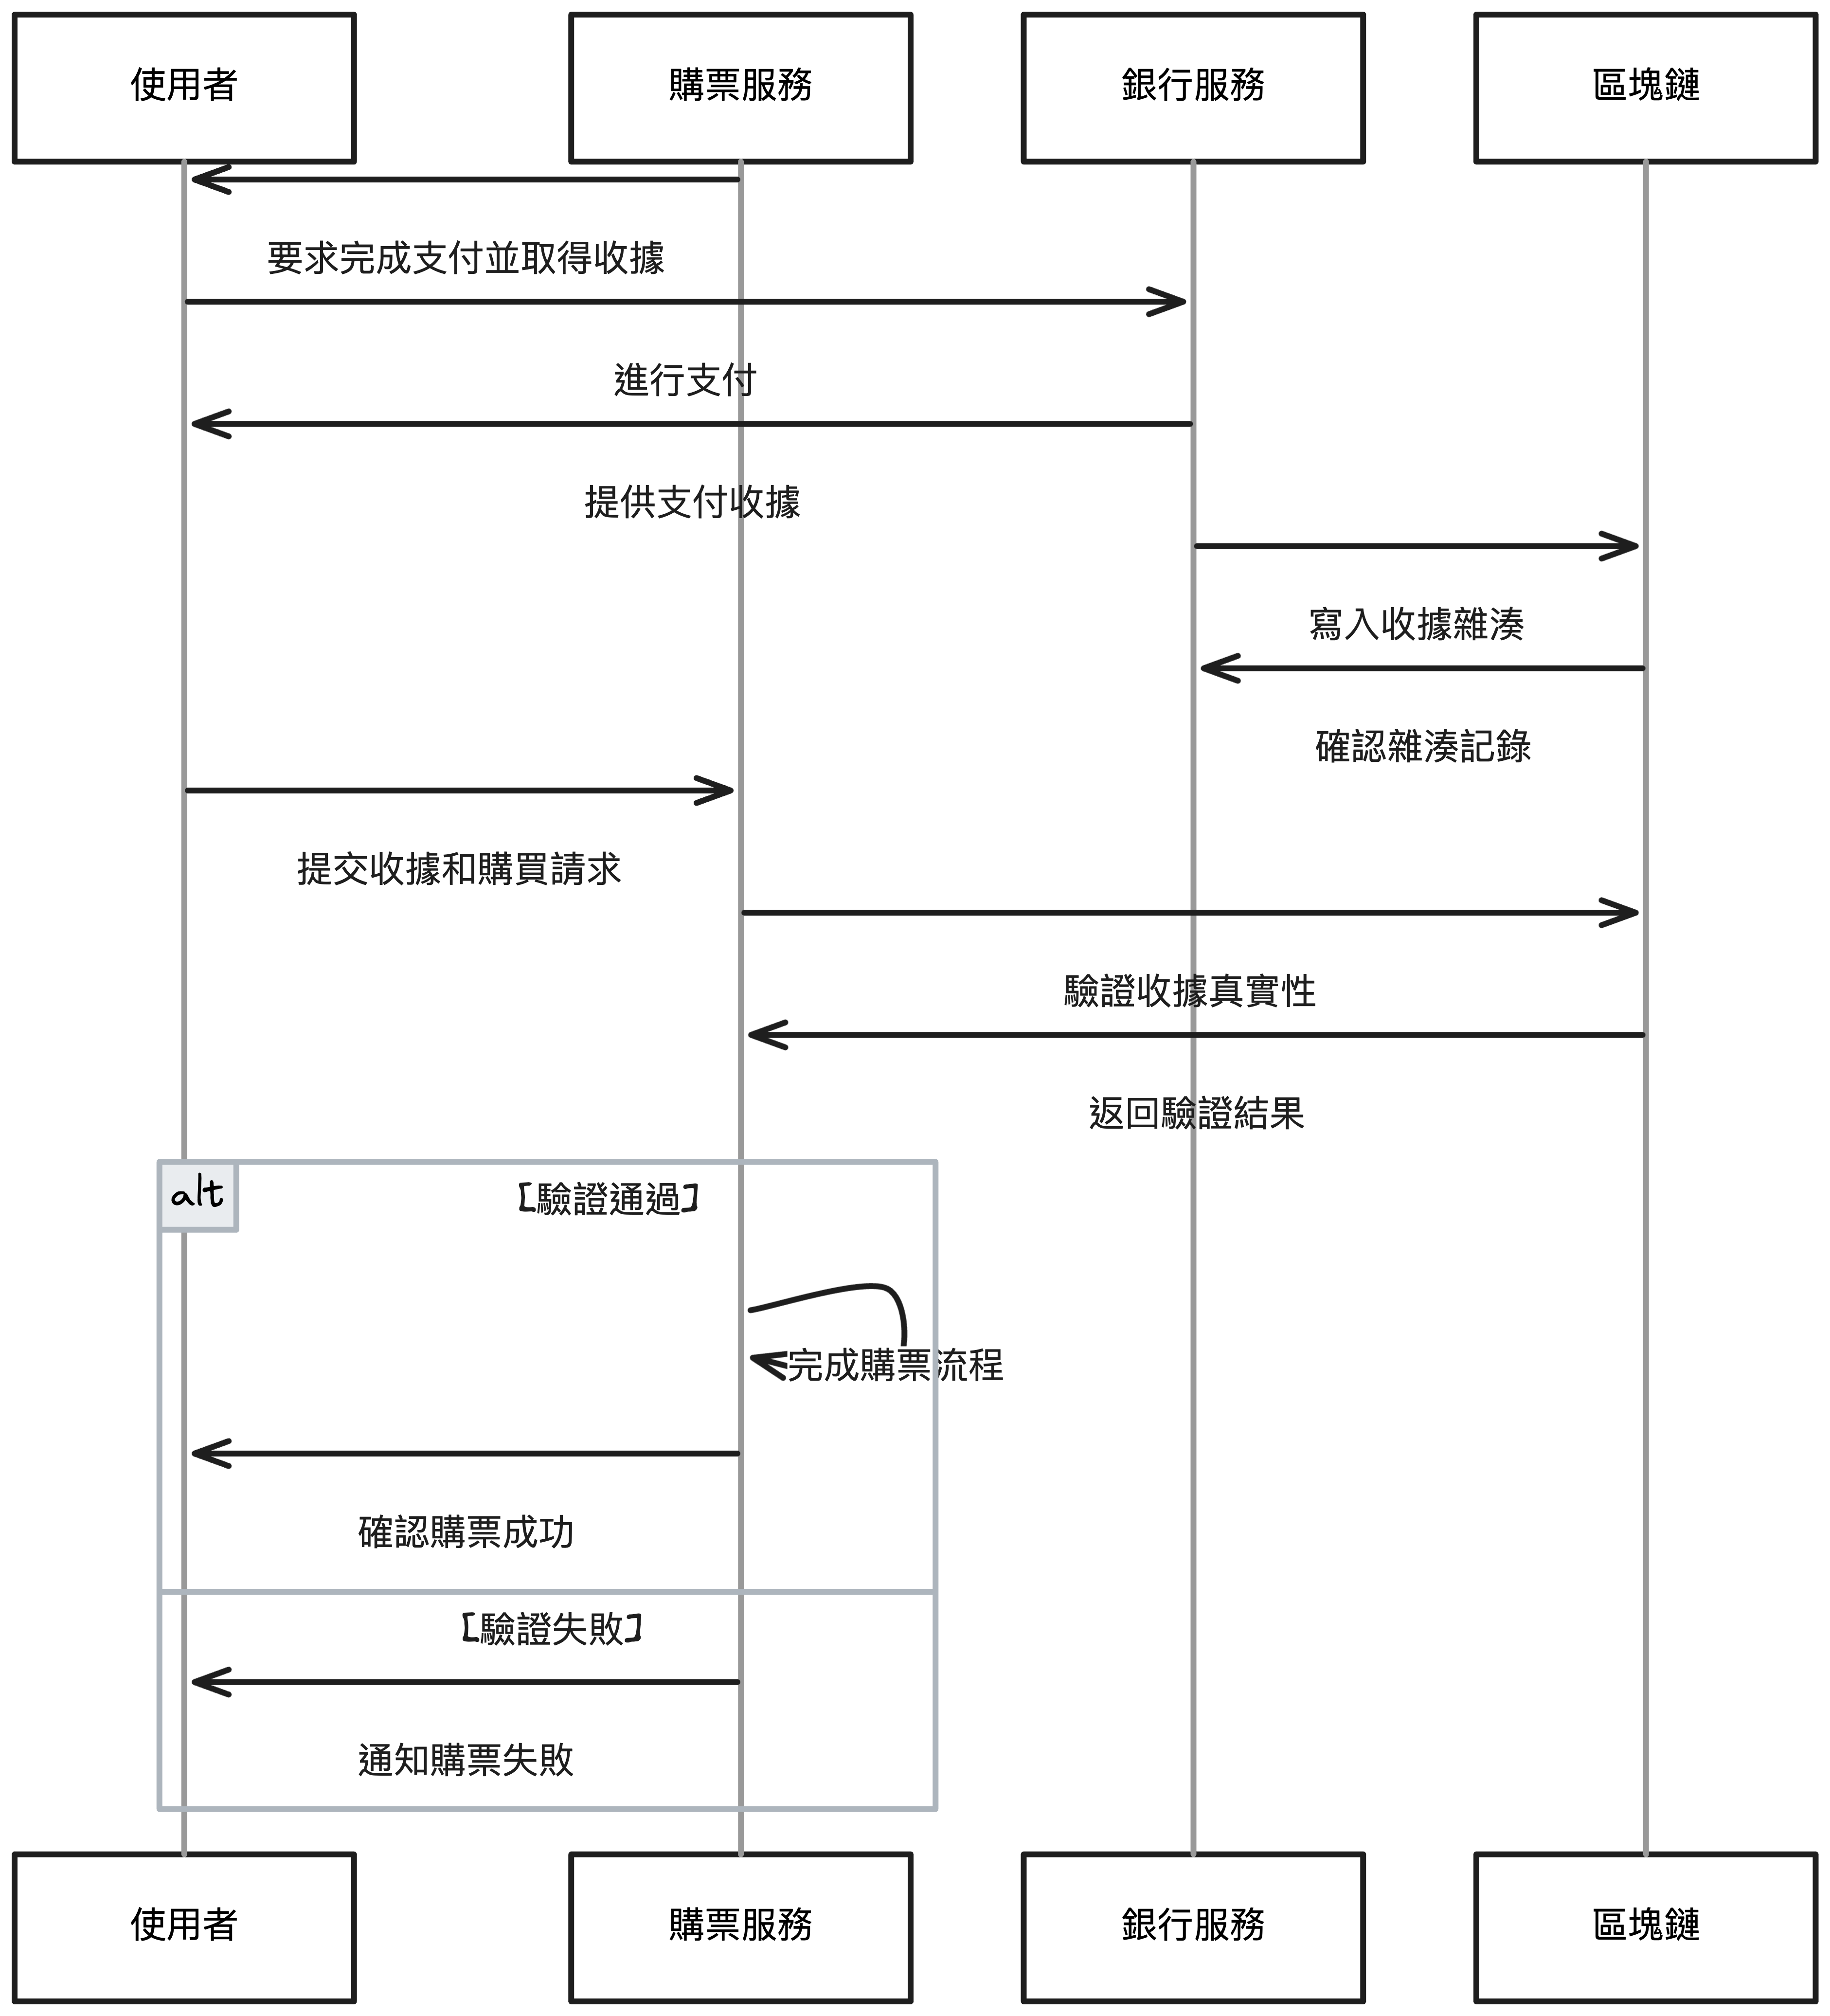
\includegraphics[width=\linewidth,keepaspectratio]{figures/flow-3-part.png}
  \caption{跨服務共識流程}
  \label{fig:flow-3-part}
\end{figure}
舉例來說,實作一個使用第三方支付服務的購票系統時,本研究的方法與現行的網路後端設計\ref{fig:flow-3-part-0}有所不同。現有設計中,支付系統全權負責與相關服務的串接,使用者僅需與支付系統溝通。而在本研究提出的架構中如圖\ref{fig:flow-3-part},流程如下:
\begin{enumerate}
  \item 購票系統要求使用者到銀行服務完成支付並取得收據。
  \item 銀行服務將收據的雜湊寫入區塊鏈。
  \item 使用者向購票系統提交收據和購買請求。
  \item 購票系統在區塊鏈上驗證收據的真實性。
  \item 驗證通過後,完成購票流程。
\end{enumerate}
這種設計方式將使用者置於服務提供者之間,使得使用者能夠自主控制整個支付流程,充分展現了自主身分系統的核心理念。

儘管這種方法為基於AID的微服務架構中的數據管理提供了安全且靈活的解決方案,但仍存在一些需要進一步研究的問題。例如,在大規模系統中如何優化區塊鏈性能以支持高頻率的數據更新,如何使這種技術方案符合不同國家和地區的數據保護法規,以及如何讓使用者的個人裝置成為橋樑,主動從眾多服務中選出目標並進行串連。這些都是未來研究的重要方向。

總的來說,通過結合數據憑證和區塊鏈技術,這種方法為微服務架構中的數據管理提供了一個既安全又靈活的解決方案,尤其適用於需要高度數據完整性和即時性的應用場景。隨著技術的不斷發展和完善,這種方法有望在未來的分布式系統設計中發揮更大作用,為數據的安全傳輸和管理提供新的模式。
\subsubsection{無特權的執行}
本研究認為無特權的執行也是AID系統必要的一環,因為即使服務提供者有著最好的意圖,但是只要存在特權管理者,就意味著使用者還是被迫要信任他人。但是,要求使用者擺脫對管理者的依賴絕非易事,因為這會導致使用者需要完全對自己的行為負責,例如不可以遺失密碼、不可以被盜用等,這樣的要求對於大多數使用者來說是不切實際的。

因此,本研究提出基於「極限多因素驗證」的暫時提權方案,當使用者需要執行某些特權操作時,服務會要求使用者用更多個驗證因素證明自己,以此達成更高的可信度。這樣的設計不僅可以讓使用者自主管理自己,也可以盡可能維持使用者的便利性與認知範圍。
\subsection{信用評分}
在過去的AID系統設計中,每個AID的角色(actor)都會在AID Server中被服務提供者評價,而所有系統參與者都可以查詢這些評價,藉此判斷對方的信用與真實性。然而,本研究認為這樣的做法存在問題如下:
\begin{enumerate}
  \item \textbf{整個系統的信任,而非對使用者信任:} 評價機制僅針對使用者的行為,忽視了服務提供者的信用,而後者實際上更需要受到關注。
  \item \textbf{尊重個人的道德標準:}系統參與者無法自主決定如何被評價或如何評價他人,評價方法與標準完全由AID Server制定。這與AID中「自主量化」的目標相悖。
  \item \textbf{AID生態的建立:}整個信用系統的維運方式存在問題。AID系統需要一個完整的生態系統才能長期運行這樣的信用評分機制。
\end{enumerate}
為了解決這些問題,本研究提出了一個基於區塊鏈的信用評分機制,這個機制將信用評分的權力交還給使用者,讓每個參與者都可以自主決定自己的信用標準。這樣的設計不僅可以提高系統的透明度和公正性,還可以激勵參與者更積極地參與到AID生態中來。
\subsubsection{信用評分機制}
本研究把整個自主身分系統視為一個去中心化自治組織(DAO)。每個系統參與者(包含服務供應者和終端使用者)都擁有自己的標準來基於評價判斷信譽,同時每個參與者也有權決定自己應該如何被評價。為了實現這一目標,本研究提出了完整的流程來描述評價與信譽轉換:
\begin{enumerate}
  \item \textbf{產生憑證:} 系統參與者創建「數據憑證」或「自主憑證」後,可以把對應雜湊放在自己決定的智能合約中上鏈,這個智能合約可以自訂許多規則,如是否允許別人對憑證進行評價,又或是評價的格式或條件等。所以,在本研究設計的AID系統中,使用者如果要允許評價,必須要把個人不同的角色資料(actor profile)轉換成憑證上鏈。
  \item \textbf{產生評價:} 取得明文憑證的人可以在區塊鏈上找到對應的智能合約,根據合約的規則對憑證進行評價。評價的內容必須遵循智能合約的規則,否則無法上鏈。
  \item \textbf{信譽轉換:} 用有明文憑證的人找到對應智能合約後可以讀取評價列表,之後根據自己認同的計算標準或演算法將評價轉換為信譽值。這個信譽值可以用於後續的信任判斷。
\end{enumerate}
進一步來說,一些使用者可能希望根據評價者的信譽值來調整每條評價的權重,以更有效地防範惡意評價。但是,設計此功能並非易事。它可能需要引入評價者作為系統中的新角色,並考慮如何綜合多個評價者的評分結果\cite{josang2006exploring}。最後,還需要考慮如何通過智能合約來實現這些複雜的功能。
\subsubsection{生態系的營運}
智能合約作為AID核心的信任機制載體,需要同時思考DAO治理的問題,這涉及到區塊鏈的經濟模型。本研究提議在區塊鏈中發行一種逐漸增加的自主身分統治代幣。這種代幣可被抵押,用於創建使用者的自主身分,藉此防止惡意使用者大規模創建惡意帳戶。每個自主身分(相當於其背後的代幣)可參與定期投票,討論評價機制的調整、新的智能合約協議等議題。為確保區塊鏈的長期運作,本研究建議對失去信任的使用者實施懲罰,同時獎勵基礎設施的運作。因此,用於創建自主身分的代幣抵押後不可贖回,被鎖定在區塊鏈上。因此,可以確保使用者不會輕率創建自主身分,並激勵使用者維護自身自主身分的信譽。此外,本研究建議對使用者在鏈上的每項操作採取使用者付費模式,使區塊鏈的維護者能獲得報酬,從而保證區塊鏈的持續運作。
\section{系統架構設計}
基於上述核心機制,本研究提出了一個完整的自主身分系統架構。這個架構融合了系統的技術層次和參與者角色,形成了一個統一且高效的生態系統。本節將詳細介紹這個架構的結構和設計理念。
\subsection{系統結構概覽}
\begin{table}[h]
  \centering
  \begin{tabular}{|c|c|c|}
    \hline
    層次  & 角色    & 主要功能              \\
    \hline
    共識層 & 共識核心  & 提供可信賴的數據讀寫機制      \\
    \hline
    服務層 & 服務提供者 & 提供特定服務,不直接儲存使用者資料 \\
    \hline
    數據層 & 終端使用者 & 管理個人數據,使用服務       \\
    \hline
  \end{tabular}
  \caption{自主身分系統層次與角色對應}
  \label{tab:system-layers}
\end{table}
自主身分系統架構包含三個層次,由上到下分別是共識層、服務層、數據層,每個層次對應一種關鍵角色分別是共識核心、服務提供者、終端使用者。這種對應既反映了系統的技術架構,也體現了各參與者在系統中的功能和職責。圖\ref{fig:aid-system-layer}展示了這種層次-角色對應關係,表\ref{tab:system-layers}則展示了各自的存在目的。
\begin{figure}[h]
  \centering
  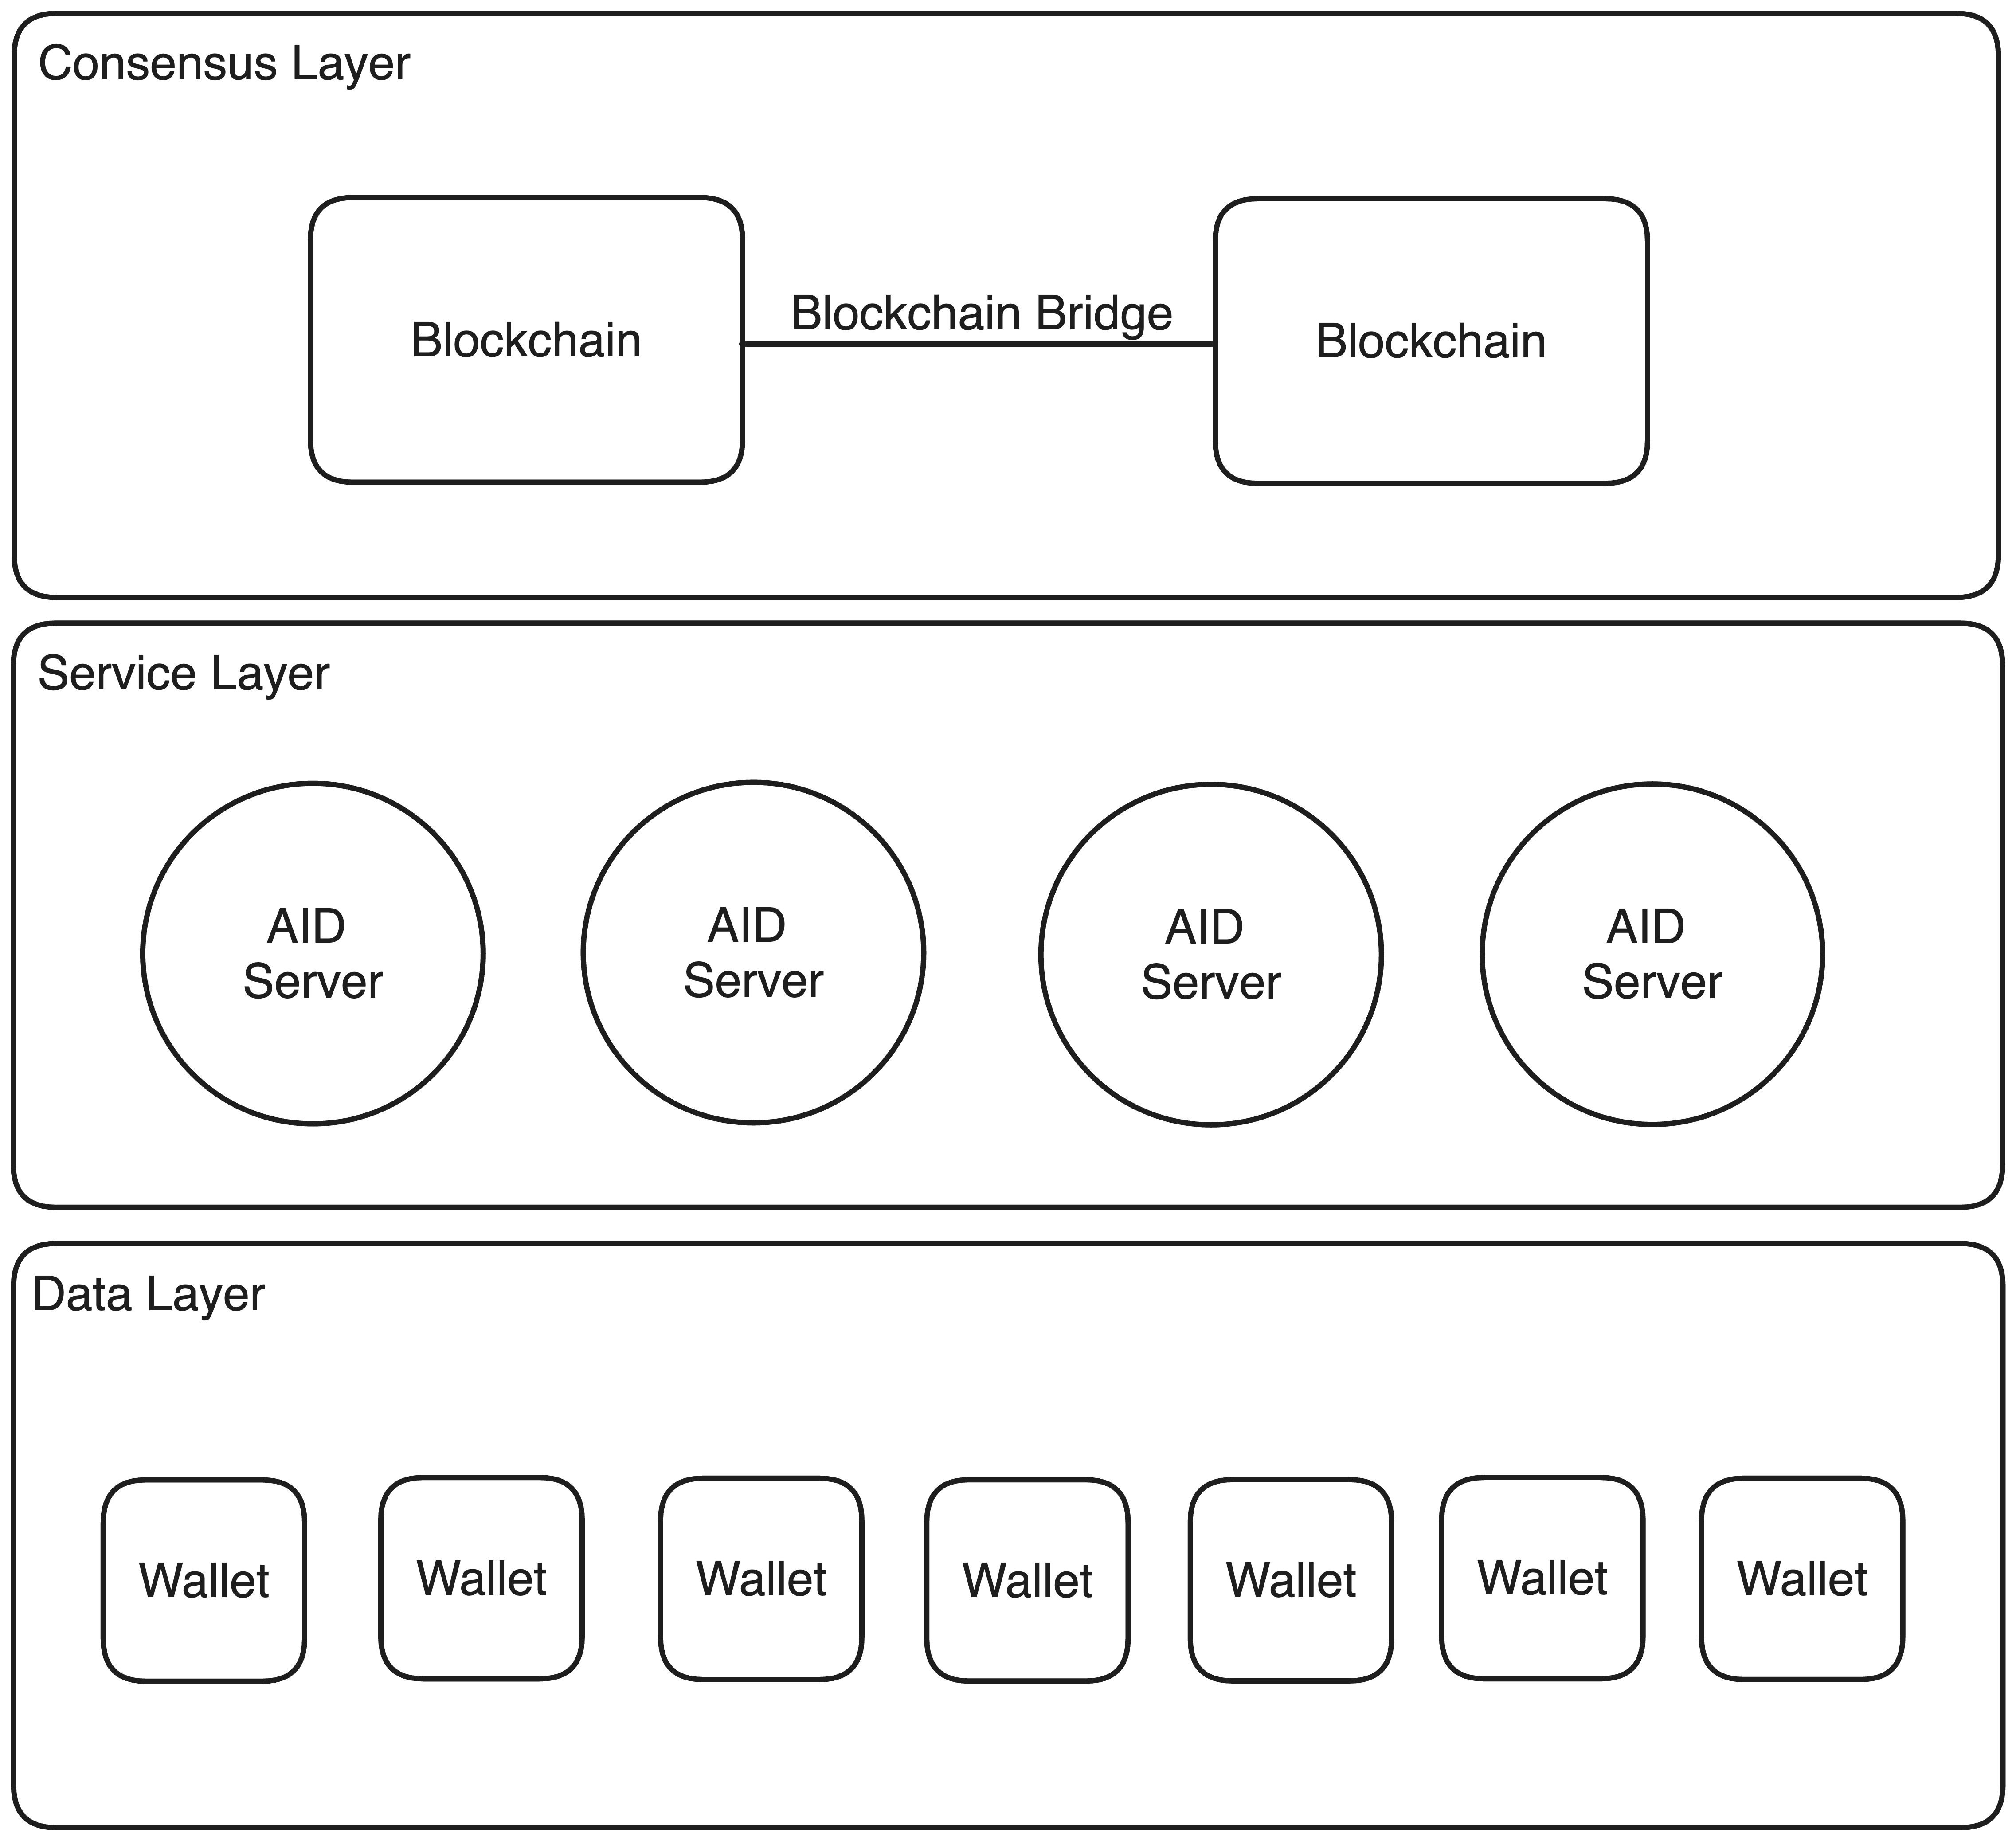
\includegraphics[width=\linewidth,keepaspectratio]{figures/aidLayers.png}
  \caption{自主身分系統結構圖}
  \label{fig:aid-system-layer}
\end{figure}
\subsection{層次與角色對應}
自主身分系統是個龐大的系統,每個層次內可以包含多個能平行擴展的角色實作,因此為了確保各個層次的模組化、易抽換、可擴展、靈活、安全和互操作等優勢,本研究明確訂出了各層的功能和職責。
\subsubsection{共識層與共識核心}
共識層在自主身分系統中扮演著基礎設施的角色,其主要參與者是共識核心。共識核心通過提供可信賴的數據讀寫機制,確保了「數據憑證」與「自主憑證」等機制在達成共識方面的可能性。其設計目的是確保數據的一致性和可信度,為整個系統提供堅實的信任基礎。共識層的實現可以靈活選擇,既可以採用區塊鏈技術,也可以使用其他形式的共識機制,以滿足不同場景的需求。
\subsubsection{服務層與服務提供者}
服務層是系統的中間層,對應的參與者是各個服務提供者。每個服務提供者都提供特定的服務,並且可以通過符合AID系統標準的介面加入系統。服務提供者不直接儲存使用者資料,而是作為使用者聚集的節點,使用者能夠自由地利用AID系統使用所需的服務。這種設計既保護了使用者數據隱私,又提供了靈活的服務串接機制。
\subsubsection{數據層與終端使用者}
數據層是系統的應用層,直接面向終端使用者。在這一層中,每個終端使用者擁有自己的數據存儲空間,並且系統提供了一個統一的數據管理介面。使用者可以自由地管理自己的數據與身分,並且通過「數據憑證」與「自主憑證」機制來獲得他人對個人身分或數據的信任。
\subsection{共識層}
共識層是自主身分系統的基礎建設,主要由無數個共識核心組成。共識核心內包含無數個憑證,不管是「數據憑證」還是「自主憑證」。當共識核心由區塊鏈實作時,會使用智能合約來實現憑證的寫入、讀取、更新和評價等功能,分別介紹:
\begin{itemize}
  \item \textbf{寫入:} 用於合約初始化,將數據對應的雜湊與公開資訊寫入合約狀態。
  \item \textbf{讀取:} 讀取合約狀態中的雜湊或公開資訊,用於驗證或查詢。
  \item \textbf{更新:} 由憑證擁有者執行,用於即時變更憑證狀態,如撤銷或停用。
  \item \textbf{評價:} 允許使用者根據智能合約規則,以特定格式讀取或寫入評價內容。
\end{itemize}
為了更好地理解共識層的運作,以學歷驗證為例。在這個場景中,使用者向學校申請學歷證明,學校將證明的數位雜湊寫入區塊鏈。任何需要驗證該學歷的服務都可以通過讀取區塊鏈上的雜湊來確認其真實性。若使用者的學歷狀態發生變化,學校可以即時更新區塊鏈上的雜湊狀態,確保驗證方獲得最新資訊。此外,如果某企業對學歷證明的可信度存疑,可以在區塊鏈上留下評價,供其他驗證方參考。
\subsection{服務層}
服務層是自主身分系統的應用層,負責提供各種服務。自主身分系統不包含具體服務的實作,只是提供名為AID Server的後端SDK規格,讓服務開發者能夠輕鬆地把自己的應用串接自主身分系統。本研究設計了AID Server的幾個關鍵功能:
\begin{itemize}
  \item \textbf{身分管理:} 提供服務加入、登入、登出等基本身分管理功能。
  \item \textbf{憑證管理:} 提供憑證的創建、更新、讀取、評價等功能。
  \item \textbf{數據管理:} 提供使用者數據的導入、導出等功能。
\end{itemize}
以下將分別介紹這幾個功能的設計細節。
\subsubsection{身分管理}
對服務提供者而言,新的自主身分加入必須先由使用者上傳「自主憑證」。此時,服務提供者可選擇是否接受該新自主身分。多數公開服務可能接受任何自主身分,但私人服務或有更高要求,如僅接受特定機構簽章的自主憑證,或基於評價機制被充分信任的自主身分。一旦服務提供者接受新的自主身分,該身分即可開始使用服務。

為了在確保安全的同時提供便利,自主身分系統提供了兩種登入方式:簡易登入和多因素驗證登入。簡易登入是指使用者僅需提供少量資訊即可登入,如使用者別名和密碼。多因素驗證登入則要求使用者提供更多資訊,如電子郵件驗證碼、手機簡訊驗證碼或私鑰等。服務提供者可根據自身需求選擇是否啟用簡易登入功能。

另外,儘管自主身分(AID)的生成是透過UUID機制\cite{uuid}產生唯一識別號,但AID系統允許使用者在服務中設定自己偏好的別名,而非如傳統身分服務限制使用唯一的電子郵件地址作為使用者名稱。在日常操作中,系統優先讓使用者使用別名作為帳號完成簡易登入,只有當別名難以被識別時,才會要求使用者使用與UUID關聯的多因素驗證登入機制進行識別。本研究認為該設計更能表現出使用者對自己身分的自由控制權。

最後,服務提供者應當實作完善的登出功能,讓使用者能夠有效管理自身的在線狀態。這一功能不僅允許使用者標示自己的當前狀態,更應包含請求服務端遺忘所有數據和終止會話(session)等選項。因為在自主身分中,使用者擁有自己的數據,服務提供者僅提供服務,因此每個使用週期結束後,服務提供者應當刪除所有與該使用者相關的數據。通過提供這種全面的登出機制,服務提供者能夠進一步強化使用者對其身分資訊的掌控,同時滿足使用者在資訊安全和隱私保護方面的需求。
\subsubsection{憑證管理}
服務層中的憑證管理包含兩個部分:分別是「自主憑證」和「數據憑證」。在「自主憑證」方面,大多數都是由使用者直接上傳,服務可以據此找到區塊鏈上使用者身分憑證的狀態與雜湊來完成身分驗證。此外,其他實體(如服務提供者或其他使用者)可基於自身經歷,在使用者憑證對應的鏈上合約中留下評價。

在「數據憑證」方面,當使用者申請共享特定數據時,服務提供者可按照預定的智能合約協議創建憑證,並將憑證發布到區塊鏈上。如果數據發生變動,服務提供者可即時更新憑證狀態,確保使用者數據的即時性和真實性。當另一個服務收到使用者在區塊鏈外提交的完整數據後,除了可以通過區塊鏈上的憑證驗證數據的真實性外,還可以在區塊鏈上留下評價,為其餘服務提供者提供參考。
\subsubsection{數據管理}
因為自主身分系統的核心在於賦予使用者控制自身數據的權利,數據管理在服務層相對簡單。理論上,服務提供者的最低要求是確保使用者能夠:
\begin{enumerate}
  \item 將當次操作所必需的數據導入服務中
  \item 在操作結束後將數據導回使用者端
\end{enumerate}
然而,這種簡單設計可能大幅降低使用者體驗。例如:
\begin{itemize}
  \item 若使用者每次操作都需要導入和導出數據,許多優化使用者體驗的功能將變得不可行,因系統無法追蹤使用者歷史數據。
  \item 頻繁的大量數據導入導出會顯著增加操作延遲和網路成本。
\end{itemize}
因此,「混合數據管理」模式成為必然選擇,即部分數據由使用者保管,部分由服務提供者保管。這種設計在保護使用者隱私的同時,也確保了操作的便利性。
然而,「混合數據管理」模式仍面臨諸多需要服務提供者與使用者達成共識的問題,包括:
\begin{itemize}
  \item 哪些數據勢必要導入服務端才能完成操作?
  \item 哪些數據可以持續保留在使用者端?
  \item 服務提供者管理的數據保留時間?
  \item 數據的使用權限?
\end{itemize}
這些問題涉及對隱私和資安的權衡,在下一節中將進一步討論。
\subsection{數據層}
數據層是自主身分系統的存儲層,負責存儲使用者個人數據。本研究設計了名為Wallet的前端SDK規格,讓數據層應用開發者能夠輕鬆地把自己的應用接入自主身分系統。Wallet的幾個關鍵功能如下:
\begin{itemize}
  \item \textbf{身分管理:} 提供自主身分的創建功能。
  \item \textbf{數據管理:} 提供使用者數據的上傳、下載等功能。
  \item \textbf{憑證管理:} 對共識雜湊的更新、讀取、評價等功能。
  \item \textbf{數據存儲:} 儲存使用者的數據。
\end{itemize}
以下將分別介紹這幾個功能的設計細節。
\subsubsection{身分管理}
Wallet 的身分管理主要提供一個核心功能:創建自主身分。這裡的創建並非指使用者加入某個服務,而是包含兩個主要功能:
\begin{enumerate}
  \item 使用者直接在本地裝置透過隨機產生的UUID創建自己的自主身分
  \item 透過「自主憑證」機制創建新的憑證
\end{enumerate}
在本研究的設計中,使用者可依據需求使用個人裝置創建不同的AID,並為不同需求生成不同的身分憑證,再利用這些憑證證明AID的真實性。當使用者需要向服務證明自己是AID的真實持有者時,僅需透過Wallet完成AID上標示的多因素驗證方案。
\subsubsection{數據管理}
Wallet的數據管理功能主要在服務需要時,將特定數據自主上傳至服務中,並在服務結束後自主下載回本地裝置。這裡的「自主」指使用者可自由選擇是否上傳或下載數據,並可自由選擇上傳或下載的數據內容。此的設計不僅更徹底地保護了使用者的安全與隱私,更因為由使用者自行攜帶數據在服務間移動,而徹底解決了數據孤島的問題。
\subsubsection{憑證管理}
Wallet的憑證管理功能主要對共識層內憑證進行更新、讀取、評價等操作。基於「數據憑證」與「自主憑證」機制,使用者與服務需要在共識層中的區塊鏈上基於智慧合約留下AID雜湊,讓人們可在區塊鏈上驗證AID的真實性。此外,所有使用者(包含服務提供者)都可在區塊鏈上對智能合約進行操作,以留下評價,藉此形成共識達成信任。

在Wallet中實作的憑證管理功能,使用者可輕易從Wallet中直接讀取共識層內的信任關係,並直接在共識層中更新自己身分憑證的狀態,以及對他人或服務的憑證評價。此設計不僅提高了使用者的自主權,更讓使用者能更直接地參與共識層的運作。
\subsubsection{數據存儲}
Wallet的數據存儲功能主要用於儲存使用者的各類數據,包括憑證、公私鑰、個人資料以及與各服務的交互紀錄等。這種設計使 Wallet成為使用者的個人化數據中心,實現統一管理。然而,將個人移動設備轉化為數據中心需解決備份、遷移和雲端儲存等問題。雖然本研究鼓勵使用者自主選擇解決方案,但仍提供以下建議實作:

每個採用自主身分系統的應用都應包含Wallet模塊,並利用設備的嵌入式資料庫存放數據。使用者可設置各Wallet的同步策略,包括自動同步(按需獲取數據)、完全同步(複製全部使用者數據)和手動同步(使用者指定數據複製)。這種設計便於實現備份、遷移和雲端儲存等功能,提升使用者數據管理的便利性。具體實現概念如下:
\begin{itemize}
  \item \textbf{遷移:} 新Wallet可通過手動輸入舊Wallet的公開地址或直接連接同一設備上的已啟動Wallet來建立連結。遷移後,新Wallet可設置對舊Wallet的同步策略。
  \item \textbf{雲端儲存:} 考慮到在單一移動設備上存儲全部個人數據的安全風險,以及終端使用者難以維護家庭點對點(Point-to-Point,P2P)集群的現實,專業雲端服務供應商可提供執行完整Wallet的服務。使用者支付費用後,可讓其他 Wallet連接到此雲端Wallet。
  \item \textbf{備份:} 當使用者在多個設備上維護多個Wallet,並重複存儲每項數據時,自然形成了數據備份機制。
\end{itemize}
這種多元化的數據管理策略不僅提高了數據安全性,也增強了系統的靈活性和使用者體驗。
\section{系統設計細節}
自主身分系統是個龐大的系統,涉及多個技術層次和參與者角色。為了更好地理解系統的運作,本節除了會深入介紹幾個關鍵技術模塊外,還會對特殊的系統流程進行詳細說明。
\subsection{區塊鏈憑證機制}
區塊鏈憑證機制是自主身分系統的重要組成部分,分成兩種憑證:「自主憑證」和「數據憑證」。能在確保隱私的同時,提供可靠的身分驗證和數據真實性驗證。以下會詳細介紹這兩種憑證的設計細節。
\subsubsection{自主憑證}
本研究參考Tze-Nan\cite{NTU202102846}提出的自主憑證概念,設計了基於區塊鏈技術的自主身分管理流程。主要概念是由使用者自行生成憑證後根據個人需求自定義憑證的內容和權限,並且擁有隨時撤銷憑證的權力。另外,憑證內可以加入使用者自訂數據,以滿足不同場景的需求。還可以把憑證傳給簽章者進行實名認證,簽章者可以把簽名放入憑證中,以確保憑證的真實性。
\begin{figure}
  \centering
  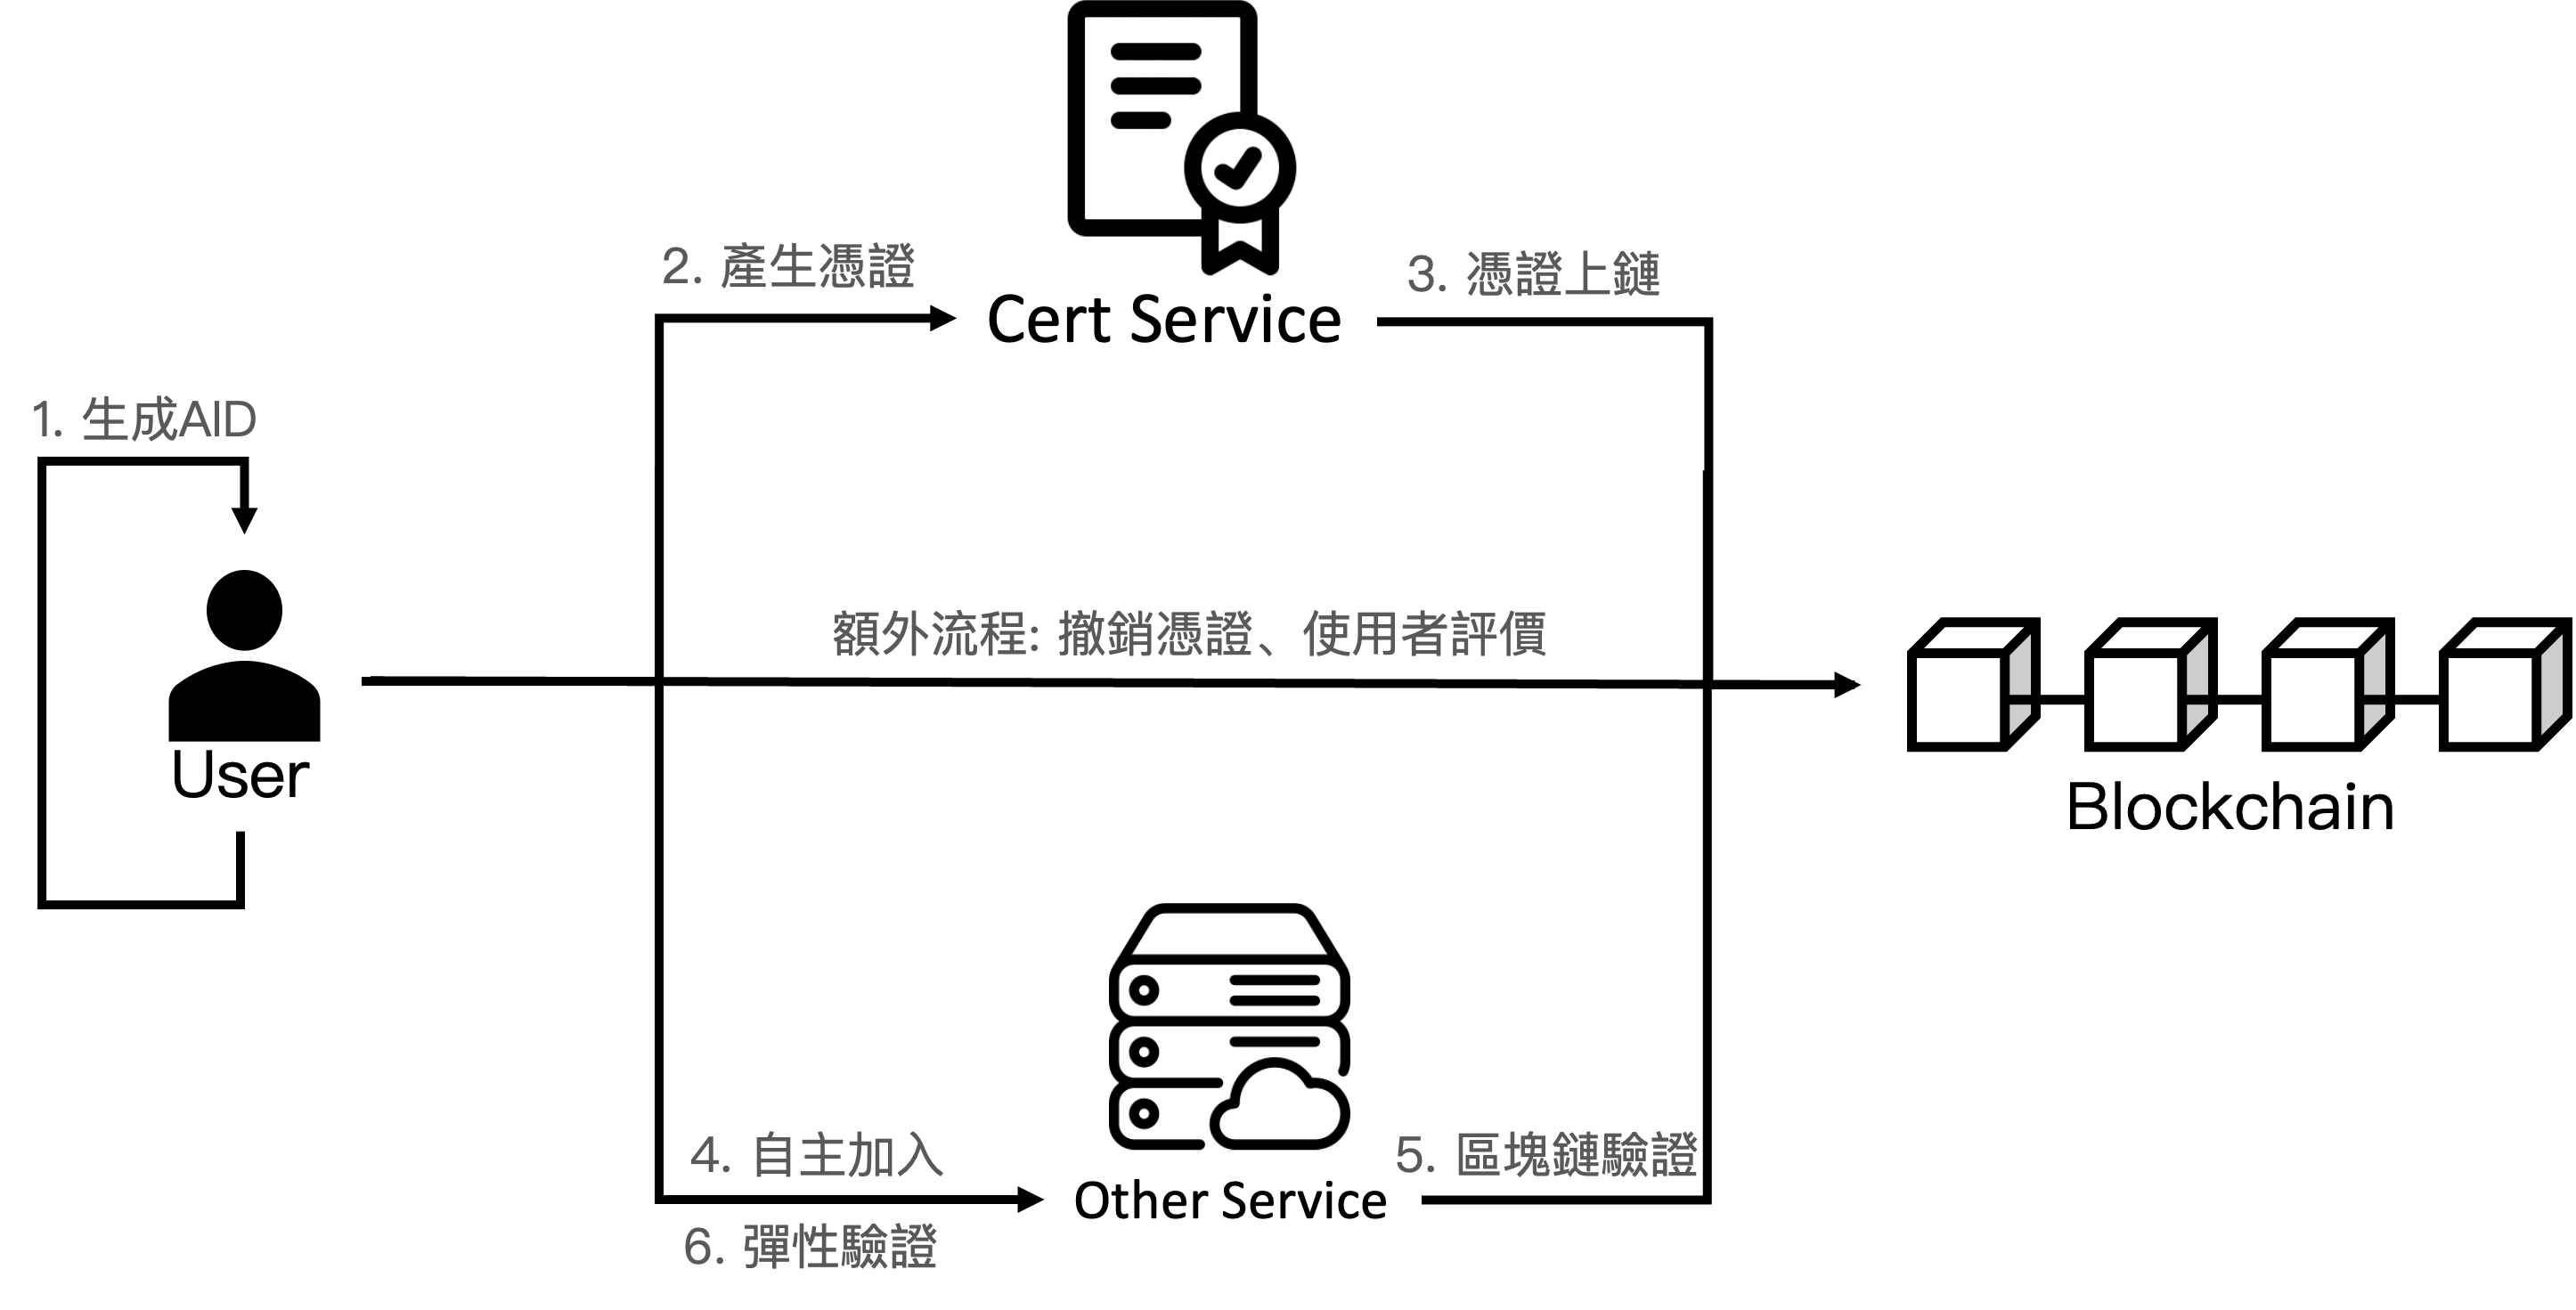
\includegraphics[width=\linewidth,keepaspectratio]{figures/flow-sc.png}
  \caption{自主憑證流程}
  \label{fig:flow-sc}
\end{figure}
本研究提出的身分管理流程包含以下關鍵步驟如圖\ref{fig:flow-sc}:
\begin{enumerate}
  \item \textbf{生成AID}:透過UUID\cite{uuid}機制離線產生唯一編號,使用者可以根據需求設置AID內含的詮釋資料(metadata),最後儲存在個人裝置中。
  \item \textbf{產生憑證}:對於實名制憑證,使用者可以將AID傳給簽章者,簽章者將AID與自己的簽名一起放入憑證中,並將憑證傳回使用者。而對於非實名制憑證,使用者可以直接在本地裝置上生成憑證,不用放入任何簽名。
  \item \textbf{憑證上鏈}:AID的雜湊(hash)作為憑證,會被簽章者記錄在區塊鏈上。
  \item \textbf{自主加入}:使用者在加入服務時,主動向服務提供者提交自己的AID,表明自己的身分。
  \item \textbf{區塊鏈驗證}:服務提供者可以在區塊鏈上取得憑證得知AID的真實性。
  \item \textbf{彈性驗證}:使用者在登入服務時,可以根據AID自主選擇多因素驗證(MFA)的方式,來取得服務的信任。
  \item \textbf{使用者評價}:區塊鏈上的憑證是AID的雜湊被放在智能合約中,相關參與者可以對憑證進行評價,從而形成該使用者的信譽。
  \item \textbf{撤銷憑證}:使用者可以隨時撤銷憑證,並在區塊鏈上自行操作。這種機制可以應用於AID外流等情況。
\end{enumerate}
此外,本系統的AID除了必須的唯一識別號,支持多樣化的metadata,以下舉例說明:
\begin{itemize}
  \item 自定義多因素驗證選項:滿足使用者登入的驗證所需。
  \item 選擇性資訊揭露:依照服務場景,使用者可以自行選擇要揭露的資訊。
  \item 設置憑證有效期限:使用者可以設定憑證的有效期限,以保護自己的隱私。
  \item 指定特定的驗證條件(如特定設備,地點或時間):增強使用者對憑證的控制。
  \item 指定特定的驗證規則(設備和網路使用限制):增強使用者對憑證的控制。
  \item 資源存取權限控制(如檔案存取權限):增強使用者對憑證的控制。
\end{itemize}

總而言之,通過這種機制提升了系統對使用者隱私和安全的保護程度,讓使用者能夠更自主地管理其身分驗證流程,保持對個人身分驗證的控制權。
\subsubsection{數據憑證}
自主身分系統中,使用者在個人設備上自行管理數據的模式引發了數據共識問題。與傳統身分系統中服務可直接調用其他服務獲取數據不同,自主身分系統在處理跨服務數據共享需求時,需要一種機制來確保數據的一致性和可信度。為此,本研究擴展了自主憑證的概念,提出了數據憑證機制。
\begin{figure}
  \centering
  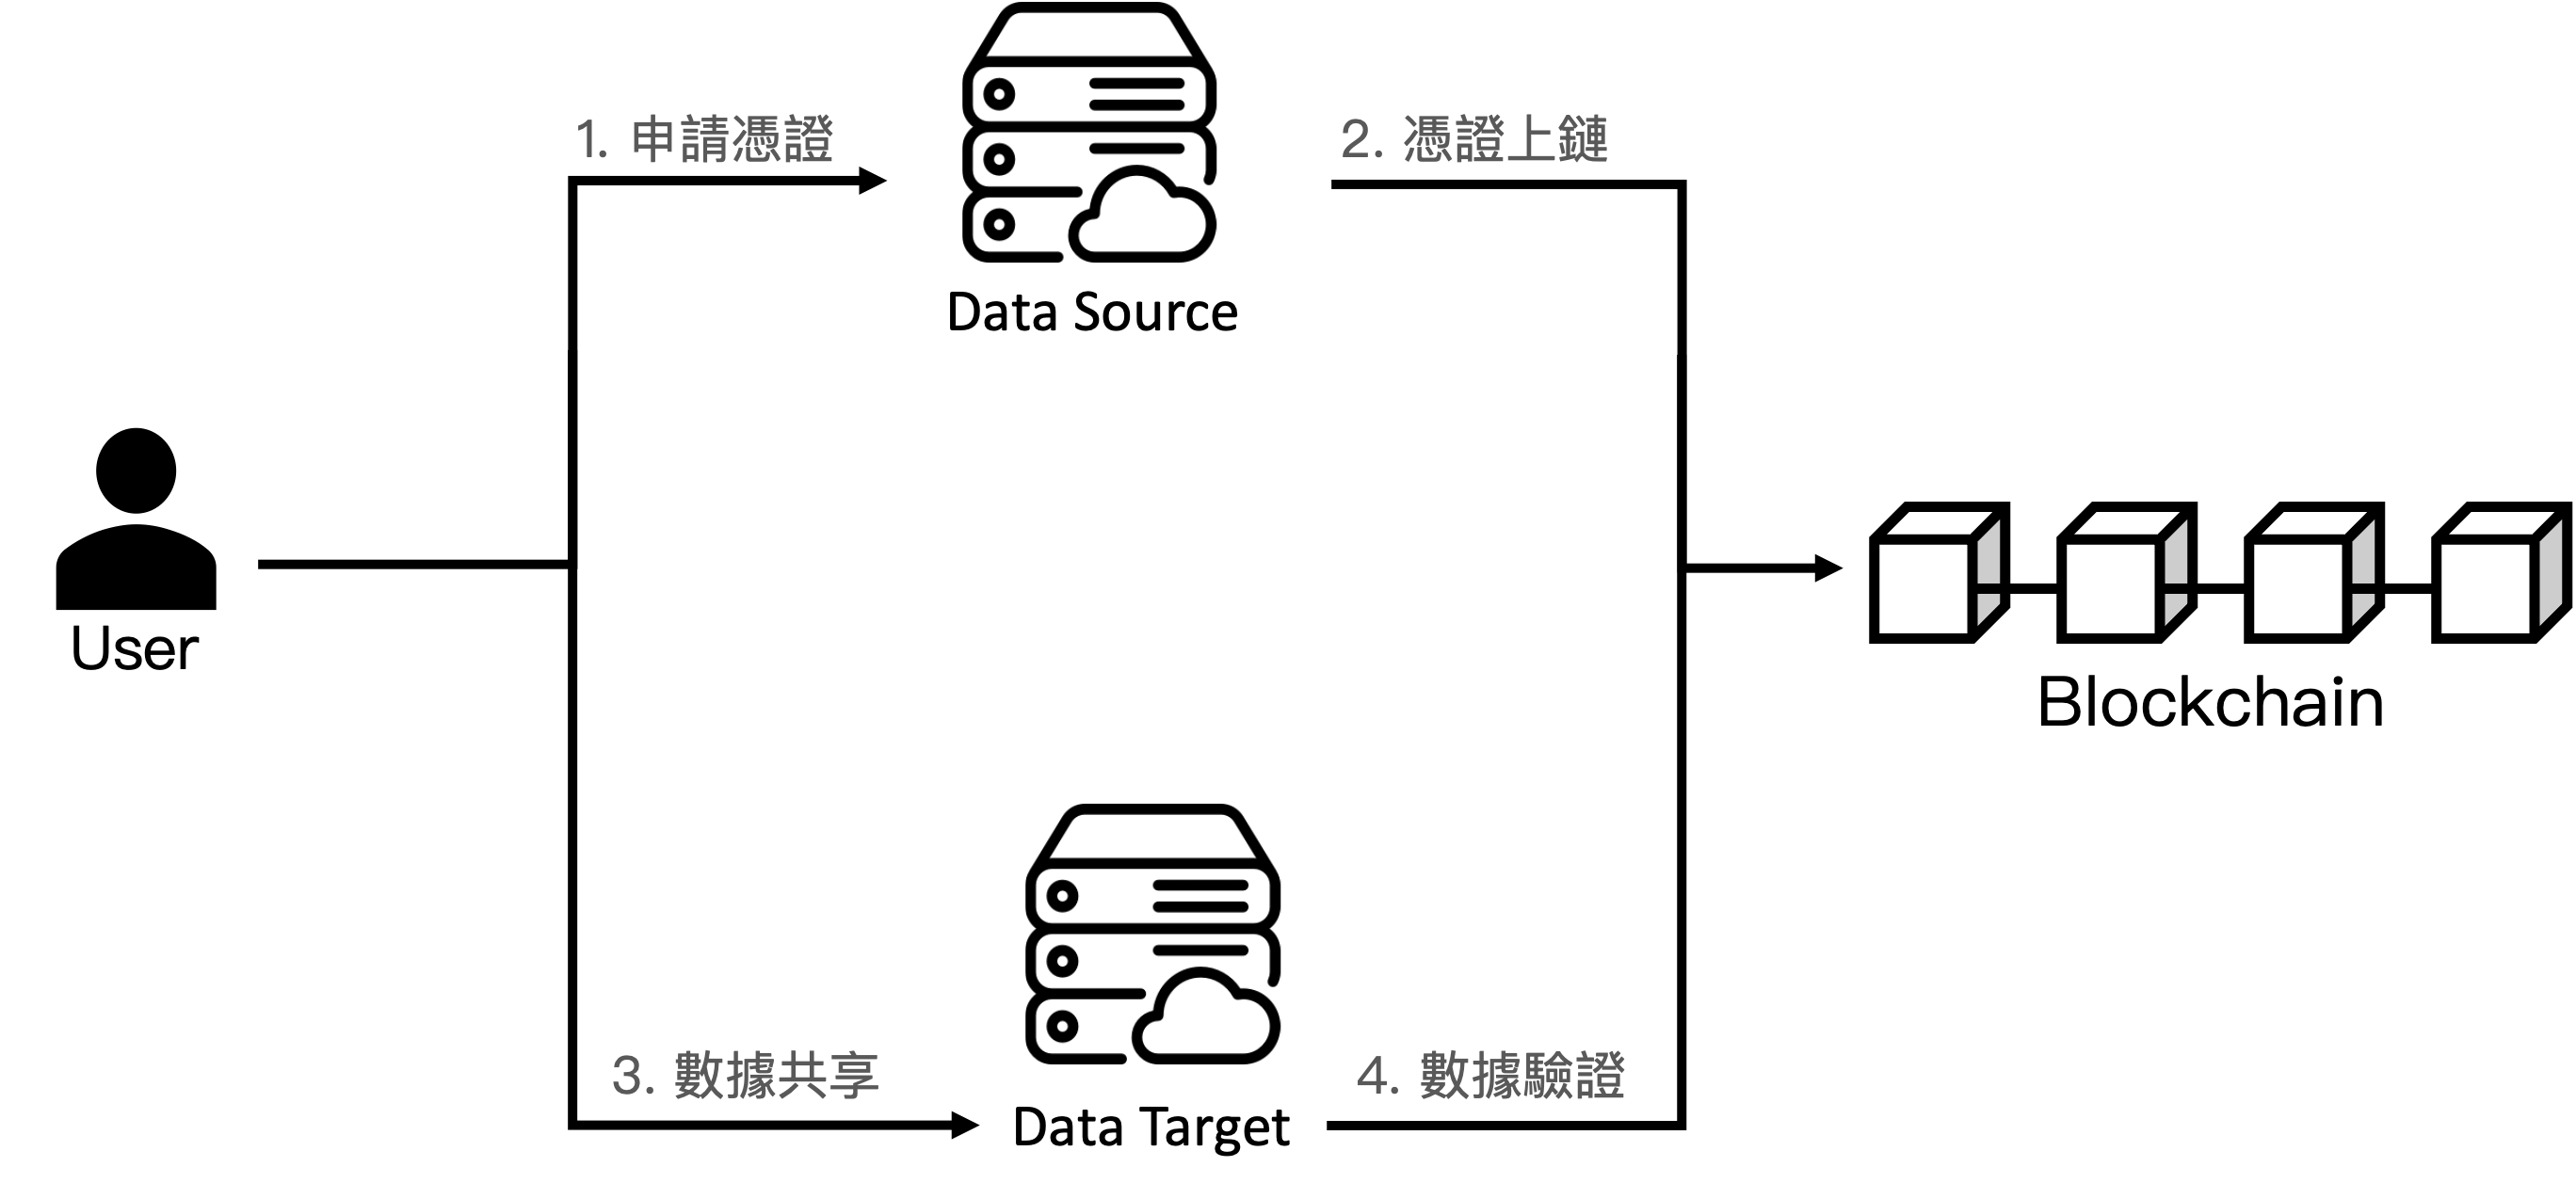
\includegraphics[width=\linewidth,keepaspectratio]{figures/flow-dc.png}
  \caption{數據憑證流程}
  \label{fig:flow-dc}
\end{figure}
數據憑證機制的運作方式如圖\ref{fig:flow-dc}:
\begin{enumerate}
  \item \textbf{申請憑證:} 當使用者需要向特定服務提交某個數據時,首先向能夠證明該數據真實性的其他服務提供者申請數據憑證。
  \item \textbf{憑證上鏈:} 接受申請的服務提供者在區塊鏈上提交該使用者數據的校驗雜湊。
  \item \textbf{數據共享:} 使用者在向特定服務提交數據。
  \item \textbf{數據驗證:} 接收數據的服務通過區塊鏈上的憑證完成數據的校驗,從而確認數據的真實性。
\end{enumerate}
這種設計讓使用者能夠在不同的自主身分服務中安全地共享數據,同時向其他使用者保證數據的一致性和可信度。

此外,數據憑證的雜湊被放置在智能合約中,允許相關使用者對該筆數據進行評價。這一做法將道德標準的概念從身分層面擴展到數據層面,進一步提高了數據的可信度和安全性。
\subsection{身分識別問題}
以自治身分為例,為了確保身分系統的去中心化,大幅度使用了區塊鏈相關技術,卻因此導致使用者體驗大幅度偏離一般使用者的需求。本研究為了解決這個問題,在自主身分系統的共識層中定義了兩種登入方法:簡易登入和多因素驗證登入。期望可以根據不同情境,讓使用者選擇登入方式,以同時滿足安全性和便利性的需求。

但是,系統該如何確保使用者能使用簡易登入方式呢?畢竟簡易登入可能因提供資訊不足而被攻擊者冒充或無法成功辨識身分。為此,本研究提出了「基於使用者時空的分析方法」,通過追蹤使用者每次操作時夾帶或產生的資訊來辨識使用者身分,並配合「基於危險程度的驗證機制」找出應要求多因素驗證的時機。

接著本研究會詳細介紹「基於使用者時空的分析方法」與「基於危險程度的驗證機制」這兩種特殊解決方案。
\subsubsection{基於使用者時空的分析方法}
每個身分本質上可視為一個隨時間變化的動態向量空間,其維度可謂無窮。每次對使用者的身分驗證都可視為取得特定時間僅含部分維度的向量。這方法的核心是讓使用者自主決定提供哪些維度,並在每次與系統互動時攜帶這些資訊。基於此概念,即讓使用者使用簡易登入,只要使用者自動攜帶裝置指紋、位置等資訊,系統即可通過比對這些資訊來進一步確認使用者身分。
\begin{enumerate}
  \item 使用者i在時間t的身分向量:
        \begin{equation}
          \mathbf{i}(t) = (i_1(t), i_2(t), \ldots, i_n(t), \ldots), \quad n \to \infty
        \end{equation}
  \item 使用者i在時間k登入時傳入的向量:
        \begin{equation}
          \mathbf{v}_k = (v_{k1}, v_{k2}, \ldots, v_{km}), \quad m \ll n, \quad v_{kj} = i_j(t_k) \text{ 對某些 } j
        \end{equation}
  \item 暫存的向量集合(假設 $\dim V = m$):
        \begin{equation}
          \mathbf{v}_k = (v_{k1}, v_{k2}, \ldots, v_{km}) \in V, \quad \dim V = m \ll n
        \end{equation}
  \item 假設相似度函數為s:
        \begin{equation}
          s: \mathbb{R}^m \times \mathbb{R}^m \to [0, 1]
        \end{equation}
  \item 身分推測方法:
        \begin{equation}
          \text{Identity} = \arg\max_{\mathbf{v}_i \in V} s(\mathbf{v}_{\text{new}}, \mathbf{v}_i)
        \end{equation}
\end{enumerate}
舉例來說:使用者在某次登入時提供了自己的別名、性別、所在地區等資訊,而在下次登入時僅提供了性別、所在地區等資訊,系統可以通過比對這兩次向量來推測使用者的別名。這種方法使使用者在不提供完整資訊的情況下,仍能通過部分資訊完成身分驗證。

然而,這種方法也帶來了一些問題。例如,使用者提供的維度多寡會影響系統的準確性,甚至使用者提供的維度是否包含可變資訊會影響系統的安全性。因此,本研究提出維度的選擇甚至各個維度的權重應由使用者自主決定,而系統僅提供推薦機制,讓使用者在不同情境下使用不同方法,以滿足其需求。
\subsubsection{基於危險程度的驗證機制}
AID系統允許使用者自定義各種行為的危險程度,並據此調整驗證的嚴謹度。然而,這種設計可能帶來兩個極端問題:過高的嚴謹度可能導致正常登入受阻,而過低則可能危及系統安全。為此本研究們提出「基於危險程度的驗證機制」希望系統性地協助使用者為不同場景設定合適的驗證嚴謹度。

這個機制建立在「基於使用者時空的分析方法」之上,綜合考慮三個關鍵因素:行為的危險程度、符合的維度數量,以及時間點的接近程度。這三者的互動決定了所需的驗證嚴謹程度。簡而言之,行為越危險,需要越嚴格的驗證;而越嚴格的驗證,則要求更多的維度符合和更接近的時間點。

值得注意的是,AID系統中,使用者可以自主決定行為的危險程度,系統僅提供建議。這種設計能滿足不同情境下的需求。例如,對於個人銀行帳戶,使用者可能將所有行為視為高度危險,因此需要最嚴格的驗證。相反,對於社群媒體帳戶,閱讀文章可能被視為低風險行為,而發布內容則可能需要更嚴格的驗證。

本研究建議使用者將危險程度定義為對數據操作的敏感度:越敏感的數據越危險,越危險的數據則需要越嚴謹的驗證機制。通過這種方式,本研究期望為各種使用場景提供既靈活又安全的身分驗證解決方案。
\subsection{密碼救援問題}
密碼救援問題是自主身分系統中的一個重要問題。在傳統身分系統中,密碼救援通常是通過中心化的機制來實現的,其本質的概念就如同系統內存在著一位管理者,共同管理著使用者的身分。但這明顯違背了自主身分追求的價值觀,因此本研究提出了「極致多因素驗證」的概念。

允許使用者在創建自主憑證時設置多種驗證方案,包括難以遺失或忘記的方法,如生物特徵識別(指紋或臉部辨識)。如此,即便使用者忘記密碼,亦可通過這些驗證方式重新取回身分。進一步擴展此方案,本研究還可以將「極致多因素驗證」概念應用於「基於危險程度的驗證機制」,根據危險程度要求使用者使用多種方法完成多因素驗證,進一步提高安全性,讓使用者即使已經被攻擊者奪取身分,也能通過補充更多項驗證的方式來取回身分。
\subsubsection{極致多因素驗證}
傳統身分驗證系統中,多因素驗證主要被視為登入時的固定驗證方案。然而,在自主身分系統的設計中,為了實現使用者功能的自由管理,人們需要一種更靈活、更強大的驗證機制,以取代傳統系統中系統管理員的角色。為此,本研究提出了「極致多因素驗證」的概念。

這一新概念的核心在於:不再將特定的多因素驗證方法視為使用者登入的唯一途徑。相反,從服務器的角度來看,每個驗證因素都應被視為使用者向服務器自主證明身分的一種方法。這種方法的靈活性體現在:
\begin{itemize}
  \item 在高風險情況下,系統可能要求連續多種因素的驗證以確保安全。
  \item 在低風險環境中,可能僅需一種因素即可完成驗證。
  \item 即便使用者遺失了某個重要的驗證因素,系統也不應將其視為無法登入,而是要求提供更多其他因素的驗證來補償。
\end{itemize}
通過這種動態和適應性的方法,極致多因素驗證不僅提高了系統的安全性,還增強了使用者的身分管理自主權,為自主身分系統提供了一個更加靈活和強大的驗證框架。
\subsection{混合數據管理}
在自主身份的理想情境中,使用者可以完全控制自己的數據,並且能夠自由地在各個服務之間移動。然而,這種情況實際上只會在極端情況下出現,即完全靜態的網頁或應用程式。這類應用不需要與外部服務進行數據交流,使用者只需下載原始碼並連接本地數據庫即可。但在現實中,這種情況幾乎不可能發生。因此,本研究提出了「混合數據管理」的概念,旨在提供一套完整的建議,讓使用者和服務提供者能夠以最簡單的流程實現最強大的安全性與隱私保護。

這種模式的核心在於:每個應用程式都應以靜態應用為基礎啟動,所有數據交互都通過Wallet模組進行,以確保統一的設計。隨後,與服務層的互動應遵循以下建議來放寬權限:
\begin{enumerate}
  \item 服務層在索取數據時應提供清晰的說明,讓使用者了解數據上傳的必要性。
  \item 採用逐步詢問的方式,協助使用者設定所有簡化的資安措施或降低的隱私保護措施。
  \item 設置應從高到低、從嚴格到寬鬆平滑過渡,讓使用者能根據自身需求調整安全性和隱私保護程度。
\end{enumerate}
此外,每次開啟權限產生數據上傳時,都可以通過「數據憑證」機制來確保數據的積極授權等問題。儘管採用這種方案仍可能因資訊上傳而產生隱私與資安問題,但從使用者流程的角度來看,它在盡可能保護使用者權益的同時,為服務提供者提供必要的數據支持,實現了雙方利益的平衡。通過這種「混合數據管理」模式,本研究能夠在自主身分系統中實現數據的高效管理,同時保障使用者的數據主權。
\subsection{組織使用者控管}
組織和個人使用者在身份控管需求上存在顯著差異,這給以使用者為中心的身份系統帶來了挑戰。傳統的身份供應商雖然為組織提供了專門解決方案,但這些方案往往會影響使用者自主性或需要額外創建身分,導致使用者反感和抵制。

AID(自主身份)系統通過「自主憑證」機制提供了一個創新方案。在這種機制下,組織作為憑證簽章者,可以在AID中明確寫入控管規則。儘管可能減少管理靈活性,但這種方法在保護使用者自主權的同時,也滿足了組織的控管需求。此外,這一機制有望推動去中心化組織的發展,為組織結構和管理模式的創新提供了新的可能性。
\section{資料結構}
本節會分別介紹自主身分系統中各角色重要物件的資料結構,以此讓讀者更清晰的了解系統的設計。
\subsection{共識核心}
共識層由不同的智能合約組成,每個智能合約都有自己的資料結構。這裡將介紹「自主憑證」和「數據憑證」機制所需智能合約的參考資料結構。
\begin{itemize}
  \item \textbf{自主身分唯一編號:} 透過UUID生成,用於識別使用者,此欄位在重視隱私的情況下可不填。
  \item \textbf{憑證操作公鑰:} 對應私鑰被註記在明文憑證中,因此智能合約可以確保操作者真的有得到實際的憑證。
  \item \textbf{憑證雜湊:} 擁有明文憑證的系統使用者可以藉此完成憑證真實性的驗證。
  \item \textbf{憑證狀態:} 用於記錄憑證的當前狀態,可能包括「正常」、「失效」、「遺忘」等。
  \item \textbf{憑證評價:} 用於記錄憑證的評價,可能包括「好」、「壞」、「中立」等,並且同時可以紀錄評價者的AID。
\end{itemize}
\subsection{AID Server}
服務層中一般會暫存使用者的明文憑證與關聯服務商業邏輯的資料結構,這裡僅介紹明文憑證的參考資料結構。
\begin{itemize}
  \item \textbf{自主身分唯一編號:} 透過 UUID 生成,用於識別使用者。
  \item \textbf{憑證操作私鑰:} 對應公鑰被註記在智能合約中,因此智能合約可以確保操作者真的有得到實際的憑證。
  \item \textbf{簡易識別方案:} 列出使用者想要使用的簡易登入方案與對應辨識內容,如「帳號密碼」、「IP綁定」等。
  \item \textbf{多因素驗證方案:} 列出使用者想要使用的多因素驗證方案與對應辨識內容,如「簡訊驗證」、「硬體金鑰」等。
  \item \textbf{個人資訊:} 用於揭露使用者願意提供的個人資訊,如「姓名」、「性別」等。
  \item \textbf{服務設定:} 用於記錄使用者希望自主設定的內容,如憑證的權限、有效期等。
\end{itemize}
拿簡易識別方案舉例,明文憑證就會包含「帳號」與「密碼」兩個欄位,而「IP綁定」則會包含「IP位址」欄位。多因素驗證方案的資料結構也類似,如「簡訊驗證」會包含「手機號碼」欄位。

另外,為了確保簡易登入的安全性,建議服務提供者暫存使用者每次識別空間與對應時間,以便透過「基於使用者時空的分析方法」來識別使用者。接著提供本研究建議的暫存資料結構。
\begin{itemize}
  \item \textbf{使用者身分:} 自主憑證明文。
  \item \textbf{使用者時間:} 用於記錄使用者每次識別的時間。
  \item \textbf{使用者空間:} 用於記錄使用者每次識別所拿到的所有數據,包含裝置指紋、IP位址等。
\end{itemize}
\subsection{Wallet}
數據層中一般會存儲使用者的所有數據,這裡介紹Wallet中的重要資料結構。
\begin{itemize}
  \item \textbf{自主身分列表} 同一個Wallet可以管理多個AID。
        \begin{itemize}
          \item \textbf{自主身分唯一編號:} 透過UUID生成,用於識別使用者。
          \item \textbf{憑證列表:} 用於記錄AID的所有憑證明文。
          \item \textbf{使用者個資:} 用於記錄AID的所有個人資訊。
          \item \textbf{使用者密鑰:} 用於記錄AID的所有公私鑰。
          \item \textbf{使用者數據:} 用於記錄AID在所有服務中的數據,以列表的形式存在,可以用服務的AID來索引。
        \end{itemize}
\end{itemize}
\section{本章總結}
為了全面評估自主身分系統相較於傳統身分系統的優勢,本研究基於前文提出的評估標準製作了以下比較表(表\ref{tab:identity-systems-comparison})。這個表格總結了本章討論的主要方面,還突出了系統和目前身分系統的差異。
\begin{table}[h]
  \centering
  \resizebox{\textwidth}{!}{
    \begin{tabular}{|p{2cm}|p{2.5cm}|p{2.5cm}|p{2.5cm}|p{2.5cm}|p{2.5cm}|}
      \hline
      \textbf{比較項目} & \textbf{中心化身分} & \textbf{聯合身分} & \textbf{使用者中心身分} & \textbf{自治身分} & \textbf{自主身分} \\
      \hline
      身分控制          & 組織控制           & 多組織共同控制       & 身分提供者控制          & 使用者控制         & 使用者完全控制       \\
      \hline
      使用者體驗         & 簡單但缺乏靈活性       & 單點登錄          & 單點登錄             & 複雜的區塊鏈操作      & 無摩擦驗證         \\
      \hline
      隱私保護          & 低              & 中等            & 較高               & 高             & 非常高           \\
      \hline
      數據存儲          & 集中存儲           & 分散在多個組織       & 身分提供者與服務         & 區塊鏈與服務        & 使用者端設備        \\
      \hline
      互操作性          & 低              & 中等            & 高                & 高             & 高             \\
      \hline
      單點故障風險        & 高              & 中等            & 低                & 低             & 低             \\
      \hline
      可擴展性          & 低              & 中等            & 高                & 高             & 高             \\
      \hline
      法規遵循          & 困難             & 較困難           & 較容易              & 容易            & 容易            \\
      \hline
      信任模型          & 中心化信任          & 聯盟信任          & 身分提供者信任          & 去中心化信任        & 自主互信          \\
      \hline
      身分證明          & 中心化驗證          & 聯盟驗證          & OAuth等協議         & 區塊鏈驗證         & 自主憑證機制        \\
      \hline
      數據共享          & 不共享            & 組織間共享         & API授權共享          & 公開數據共享        & 數據憑證機制        \\
      \hline
    \end{tabular}
  }
  \caption{各代身分管理系統比較}
  \label{tab:identity-systems-comparison}
\end{table}
通過這個比較表,我們可以看到自主身分系統在多個方面的優勢。這些優勢使自主身分系統成為一種更加易用、平等和安全的身分管理系統,有望在未來取代傳統身分系統,成為一種更加符合當今社會需求的身分管理方案。